\documentclass{article}
\usepackage{graphicx}
\usepackage{xcolor}
\usepackage{amsfonts}
\usepackage{amsmath}
\usepackage{amsthm}
\usepackage{geometry}
\usepackage{listings}
\usepackage{subcaption}

\lstset{
	basicstyle=\ttfamily,
	columns=fullflexible,
	frame=single,
	breaklines=true,
	postbreak=\mbox{\textcolor{red}{$\hookrightarrow$}\space},
}
\geometry{
	a4paper,
	total={170mm,257mm},
	left=20mm,
	top=20mm,
}
\newtheorem{theorem}{Theorem}[section]
\newtheorem{claim}[theorem]{Claim}
\newcommand{\indep}{\perp \!\!\! \perp}
\newcommand{\hb}{\hat{\beta}}


\begin{document}
	\begin{center}\LARGE\bf
		CATAM: 10.15 Variable selection and the bias-variance tradeoff (8)
	\end{center}

	%question1
	\section{}
	
	\begin{claim}
		$ \mathbb{E}_{\mathcal{T}, y|u}(y - u\hat{\beta})^2 = \sigma^2  + (u \beta - \mathbb{E}_{\mathcal{T}}[u \hat{\beta}])^2 + var_{\mathcal{T}}[u \hat{\beta}]$, where $ y \indep \mathcal{T} $
	\end{claim}
	\begin{proof}
		First, expand:
		\[\mathbb{E}_{\mathcal{T}, y|u}(y - u\hat{\beta})^2 = \mathbb{E}_{\mathcal{T}, y|u}(y^2 - 2y u \hat{\beta} + \hat{\beta}^T u^T u \hat{\beta})\]
		We know  $ y \indep \mathcal{T} $, so $ \mathbb{E}(2yu\hat{\beta}) = 2 \mathbb{E}(y)\mathbb{E}(u \hat{\beta}) = 2u\beta \mathbb{E}(u \hat{\beta}) $.
		Hence:
		\[LHS = \sigma^2 + (u \beta)^2 - 2u\beta\mathbb{E}(u \hat{\beta}) + \mathbb{E}(u \hat{\beta})^2 + [\mathbb{E}((u \hat{\beta})^2) - \mathbb{E}(u \hat{\beta})^2] \]
		\[\Rightarrow = \sigma^2 + (u\beta - \mathbb{E}_{\mathcal{T}}[u \hat{\beta}])^2 + var_{\mathcal{T}}(u \hat{\beta})\]
	\end{proof}
	
	When we remove the $ p $th covariate, we would expect a decrease in variance and an increase in bias. The irreducible variance is fixed hence would not change.
	
	Now to see this more clearly, if we take the average over the existing N tuples $ \mathcal{T} $, we get the result:
	\[\frac{1}{N} \sum_{i = 1}^{N} \mathbb{E}_{\mathcal{T}}(Y_i - X_i^T \hb )^2 = \frac{1}{N} \sum_{i = 1}^{N} (X_i^T \hb - \mathbb{E}_{\mathcal{T}}(X_i^T \hb ))^2 + \frac{1}{N} \sum_{i = 1}^{N} Var_{\mathcal{T}}(X_i^T \hb) + \sigma^2 \]
	where
	\begin{align*}
		\sum_{i = 1}^{N} Var_{\mathcal{T}}(X_i^T \hb) &= \sum_{i = 1}^{N} X_i (X^TX)^{-1} X_i^T \sigma^2 \\
		&= \sum_{i = 1}^{N} tr((X^TX)^{-1} X_i^T X_i) \sigma^2\\
		&= \sigma^2 tr(I_p)\\
		&= \sigma^2 p	\\
	\end{align*}

	So it is easy to see that if we removed the $ p $th covariate then the variance decreases.
	
	Similarly, now we look at the bias.\\
	First, assume $ \hb = \hb^{LS} $, then:
	\[\mathbb{E}_{\mathcal{T}}(X_i^T \hb ) = X_i^T (X^TX)^{-1}X^T X \beta = X_i^T \beta\]
	\[\Rightarrow \frac{1}{N} \sum_{i = 1}^{N} (X_i^T \beta - \mathbb{E}_{\mathcal{T}}(X_i^T \hb ))^2 = 0\]
	Now let $ X_i = \begin{pmatrix} X_i' \\ X_{ip} \end{pmatrix} $, $ \beta = \begin{pmatrix} \beta' \\ \beta_p \end{pmatrix} $, $ X = \begin{pmatrix} X' & \xi_p \end{pmatrix} $, where $ \xi_p $ is the $ p $th column of $ X $, so $ \xi_{pi} = X_{ip} $.\\
	So we can assume instead $ \hb = \hb^{\{1, ..., p-1\}} = (X'^T X')^{-1} X'^T Y $.
	\begin{align*}
		\Rightarrow \mathbb{E}_{\mathcal{T}}(X_i^T \hb) &= X_i^T (X'^TX')^{-1}X'^T \mathbb{E}(Y)\\
		&= X_i^T(X'^TX')^{-1} X'^T X \beta
	\end{align*}

	if $ \beta_p = 0 $, then $ X_i^T \beta = X_i^T (X'^TX')^{-1} X'^TX \beta $, hence bias remains 0.
	
	if $ \beta_p \neq 0 $, then $ X_i^T \beta = X_i'^T \beta' + X_{ip}\beta_p $, and
	\begin{align*}
		X_i^T(X'^TX')^{-1} X'^T X \beta & = X_i^T(X'^TX')^{-1} X'^T\begin{pmatrix}X' & \xi_p \end{pmatrix}\beta \\
		&= X_i^T(X'^TX')^{-1} X'^T (\begin{pmatrix} X' \beta' \\ 0 \end{pmatrix} + \begin{pmatrix} \xi_{p1} \beta_p \\. \\ . \\ \xi_{pn} \beta_p \end{pmatrix}) \\
		&= X_i^T \beta' + X_i^T(X'^TX')^{-1} X'^T\begin{pmatrix} X_{1p} \beta_p \\. \\ . \\ X_{np} \beta_p \end{pmatrix}\\
		&= X_i^T \beta' + X_i^T(X'^TX')^{-1} X'^TX_i \beta_p\\
	\end{align*}

	So $ \sum_{i = 1}^{N} (X_i^T \beta - \mathbb{E}_{\mathcal{T}}(X_i^T \hb ))^2 = \sum_{i = 1}^{N}(X_{ip}\beta_p - X_i^T(X'^TX')^{-1} X'^TX_i \beta_p)^2 $.\\
	Since these two terms are not necessarily equal, we can tell that bias increases if we remove the $ p $th covariate.
	
	

	
	
	
	%question2
	\section{}
	Refer to q2.m in Appendix (\ref{ap:q2}) and RSStrte.m in Appendix (\ref{ap:RSStrte}).
	From figure (\ref{fig:Q2_1}), we can see that as model size increases, the training error decreases. However the testing error only decreases until model size of 6, and increases after that. This is because as model size increases, the squared estimation bias decreases, but the estimation variance increases. So there is a point at which the sum is lower, before the estimation variance increase rapidly and testing error increases again. 
	
	From figure (\ref{fig:Q2_2}), we can see that with a increased training size, the training error ends up being higher than the training error from a smaller training size in figure (\ref{fig:Q2_1}), but the testing error decreases throughout as model size increases, contrary to the results in figure (\ref{fig:Q2_1}). This is because increasing training size decreases estimation variance, but squared estimation bias is not affected by increasing training set size. Hence overall the test error continue to decrease as model size increases to 10.
	
	
	%Comparing figure (\ref{fig:Q2_1}) and (\ref{fig:Q2_2}), we can see when $ N_{tr} = 200 $, the training error increases and the testing error decreases for each model size. This is because the estimation variance decreases as training size increases, which reduce testing error. Increasing training size also makes it harder to over-fit, hence increasing the training error.
	
	\begin{figure}[h]
		\centering
		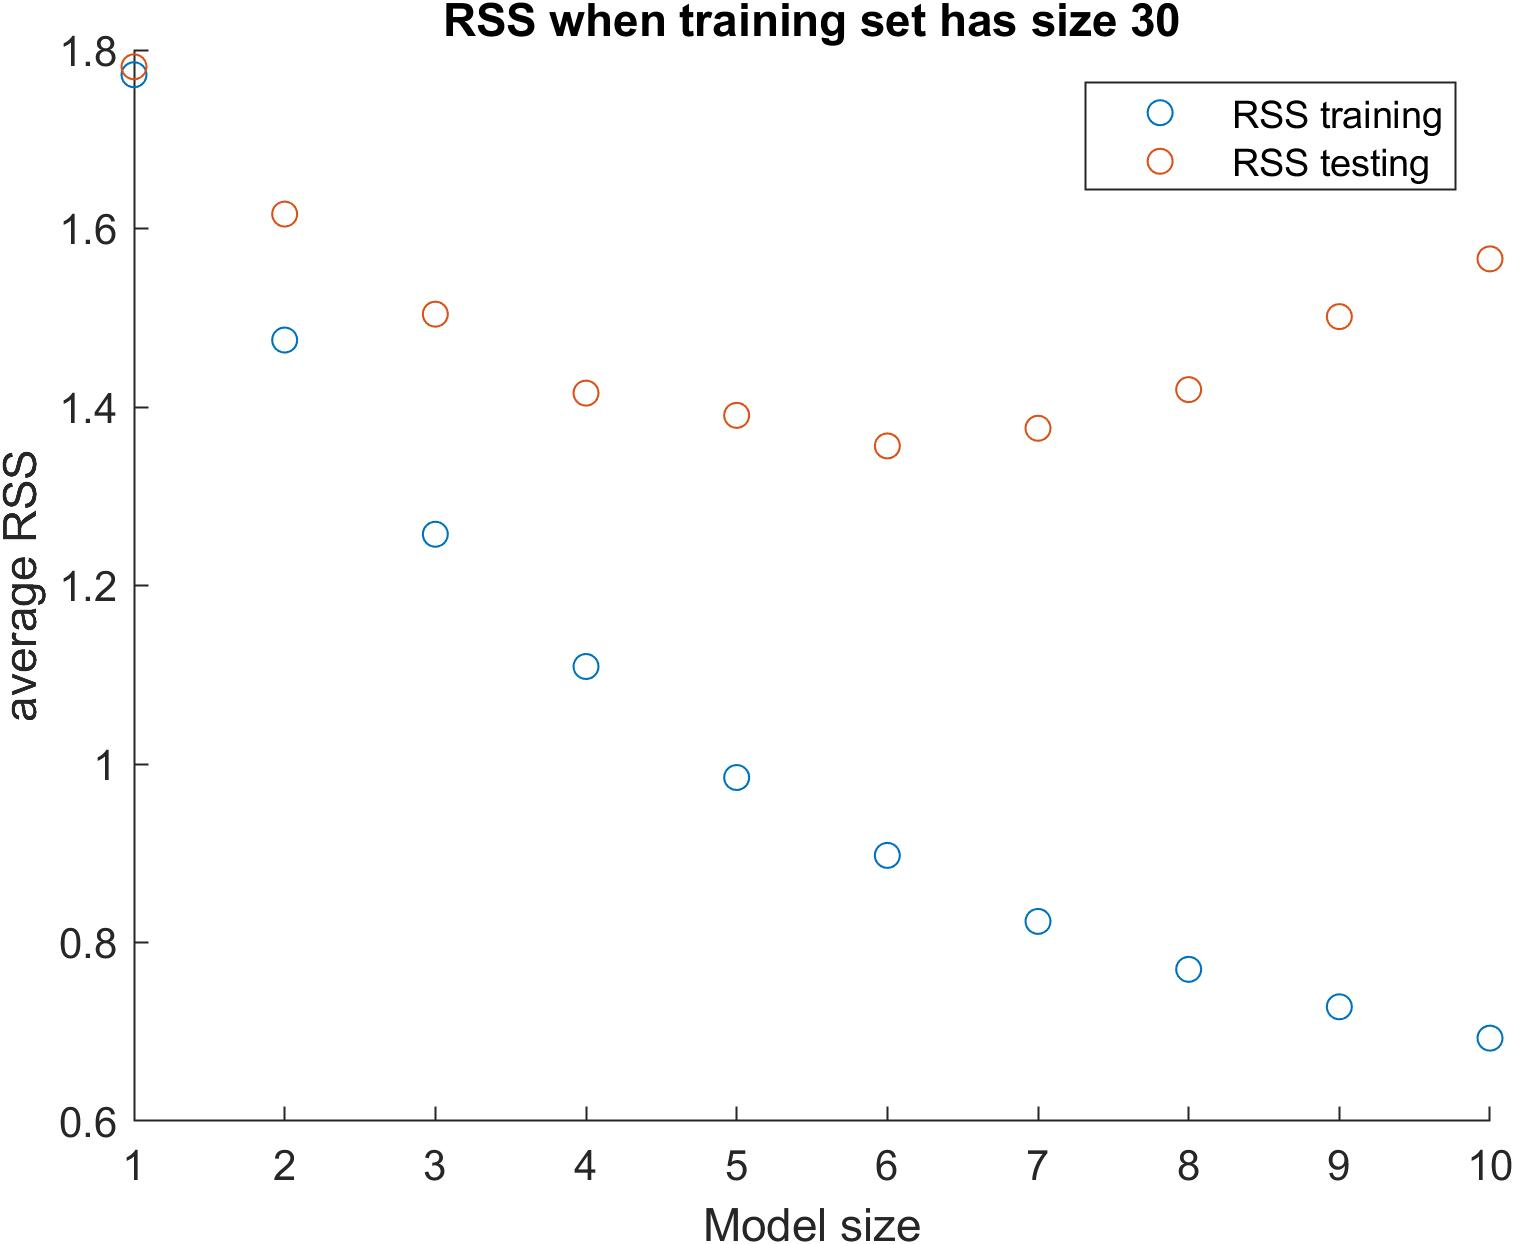
\includegraphics[scale = 0.2]{figures/q2_1.jpg}
		\caption{Average RSS against model size for training set of size 30}
		\label{fig:Q2_1}
		
	\end{figure}

	\begin{figure}[h]
		\centering
		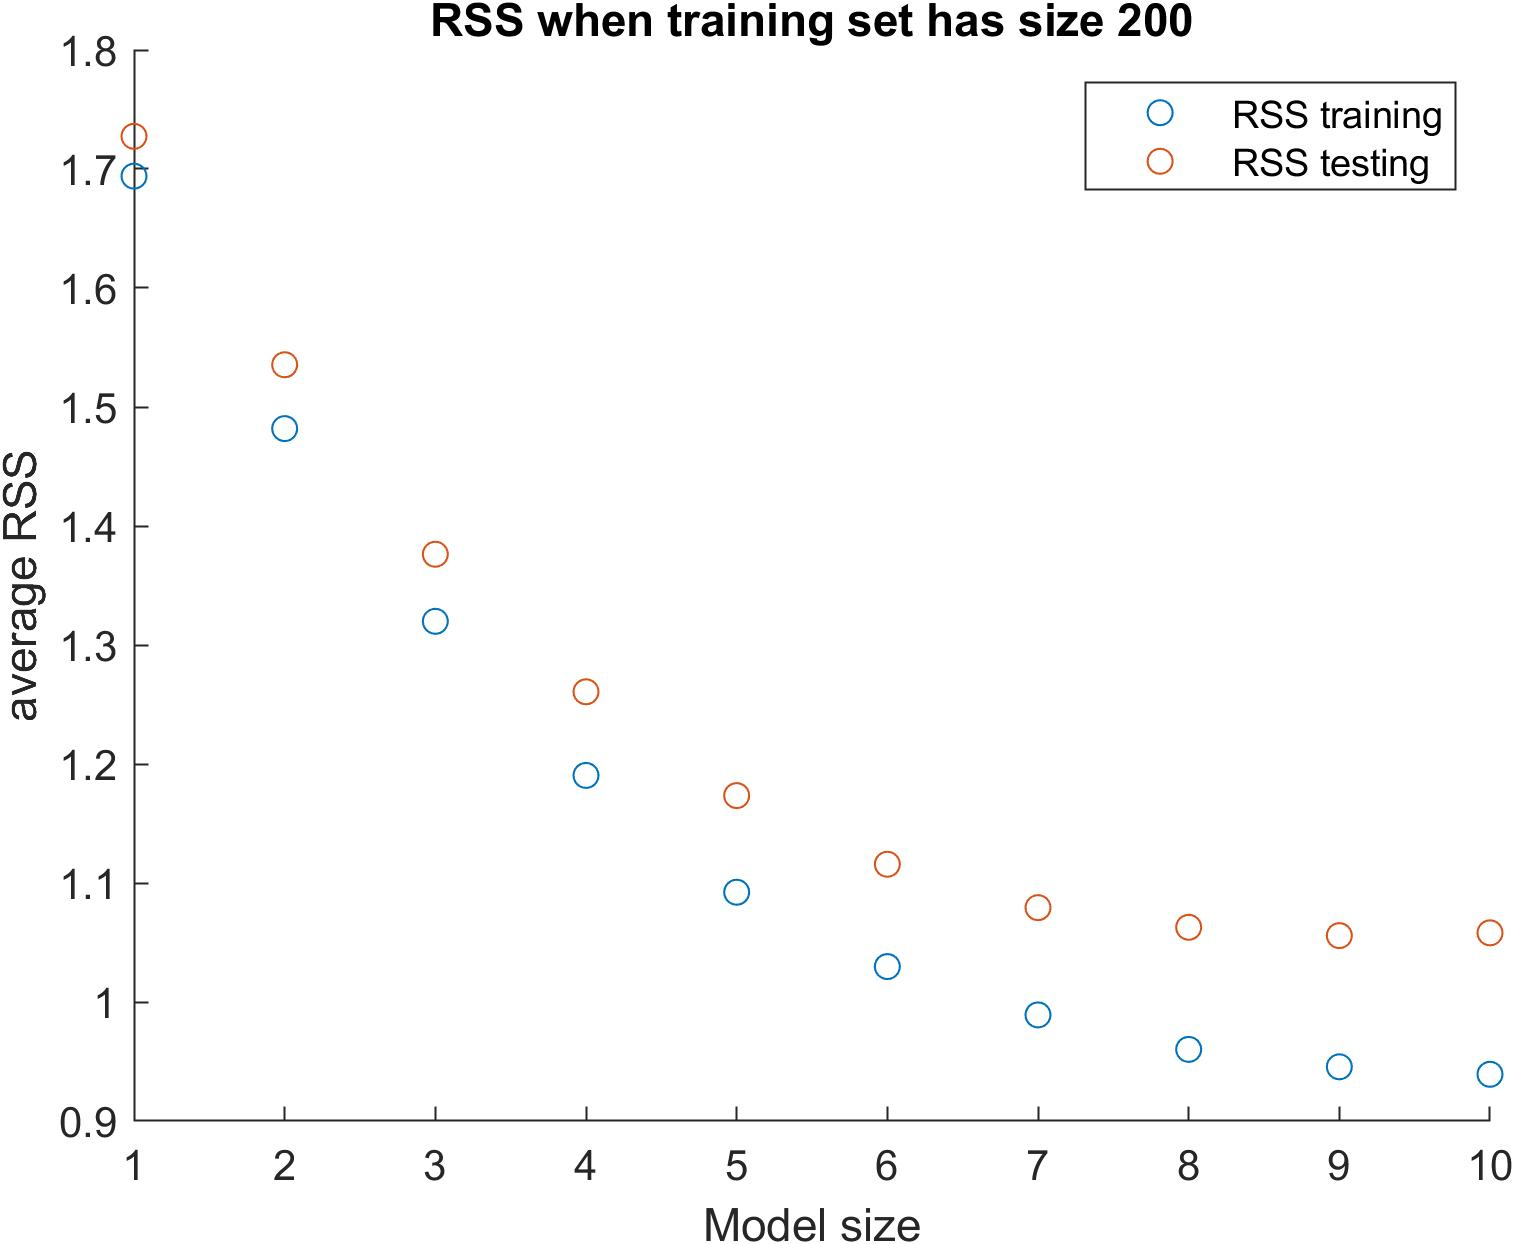
\includegraphics[scale = 0.2]{figures/q2_2.jpg}
		\caption{Average RSS against model size for training set of size 200}
		\label{fig:Q2_2}
		
	\end{figure}
	\clearpage
	%question 3
	\section{}
	Refer to q3.m in Appendix (\ref{ap:q3}), bestsubset.m in Appendix (\ref{ap:bestsubset}) and generateTrain.m in Appendix (\ref{ap:generateTrain}).\\
	Size of the model space $ \{\mathcal{M} | \mathcal{M} \subset \{1, \dots, p\}\} $.\\
	The search space $ \{\mathcal{M}| \mathcal{M} \subseteq \{1, \dots, p\}, ||\mathcal{M}|| = j\} $ has size $ \begin{pmatrix} p \\ j \end{pmatrix} $. For smallest $p$ st $ \begin{pmatrix} p \\ j \end{pmatrix} > 10^5$ for any $j$, we know choosing combination is highest when $j = \lfloor p/2 \rfloor$. 
%	So first consider the case $p$ is even: 
	We want smallest p s.t. $ \begin{pmatrix} p \\ \lfloor p/2 \rfloor \end{pmatrix} > 10^5 $\\
	%\Rightarrow \frac{p(p-1)\dots (p/2+1)}{(p/2)(p/2-1)\dots (2)(1)}$
	We can easily work out via a calculator that $ \begin{pmatrix} 19 \\ 9 \end{pmatrix} = 92378 < 10^5 $ and $ \begin{pmatrix} 20 \\ 10 \end{pmatrix} = 184756 > 10^5 $. Hence the least p such that there exists a value j for which the search space exceeds $ 10^5 $ is 20.
	
	
%	Firstly, let $ p = 2n $, we know that $\begin{pmatrix} 2n \\ n \end{pmatrix} \frac{1}{2^{2n}} = \frac{1}{2n} \prod_{j = 1}^{n-1} (1+\frac{1}{2j}). $\\
%	Also, 
%	\[\prod_{j = 1}^{n-1} (1+\frac{1}{2j})^2 = \prod_{j = 1}^{n-1} (1+\frac{1}{j} + \frac{1}{4j^2}) \geq \prod_{j = 1}^{n-1} (1+\frac{1}{j}) = n\]
%	\[\Rightarrow (\begin{pmatrix} 2n \\ n \end{pmatrix} \frac{1}{2^{2n}})^2 = \]
	%question 4
	\section{}
	Refer to q4.m in Appendix (\ref{ap:q4}), greedysubset.m in Appendix (\ref{ap:greedysubset}) and generateTrain.m in Appendix (\ref{ap:generateTrain}) \\
	Assuming $ \mathcal{M}_j = \{1, \dots, j\} $, let $ \hat{X} $ be the first j columns of the $ X $, and let $ \tilde{X} = [\hat{X}\; v] $, where $ v = X_{j+1} $. Let $ A = (\hat{X}^T\hat{X}) $ and $ \tilde{B} = (\tilde{X}^T\tilde{X})^{-1} $ Then:\\
	\begin{align}
		\tilde{B}^{-1} & = \begin{Bmatrix} \hat{X}^T \\ v^T \end{Bmatrix} \begin{Bmatrix}\hat{X} & v\end{Bmatrix}\\
		& = \begin{pmatrix}\hat{X}^T\hat{X} & \hat{X}^Tv \\ v^T \hat{X} & v^Tv\end{pmatrix}
	\end{align}
	So $ \tilde{B} = \begin{pmatrix}A & \hat{X}^Tv \\ v^T \hat{X} & v^Tv\end{pmatrix}^{-1} $
	Since A is already found from the previous iteration, there is no need to find it again. This can speed up the algorithm by reducing the number of steps needed to find $ \hat{\beta}^{M_{j+1}} $, or in fact,  $ \hat{\beta} $ for any model incrementing from $ \mathcal{M}_j $. This reduces $ N^2 \cdot j $ steps from matrix multiplication each time there is such a matrix multiplication.\\
	Each time this multiplication occurs, the order is reduced from $ \mathcal{O}(N^2) $ to $ \mathcal{O}(N) $.
	
	%question 5
	\section{}
	Refer to q5.m in Appendix (\ref{ap:q5}), greedysubsetmodified.m in Appendix (\ref{ap:greedysubsetmodified}), generateTrain.m in Appendix (\ref{ap:generateTrain}) and improvedfit.m in Appendix (\ref{ap:improvedfit}).\\
%	This would not work for best subset selection, since if 
	If we also assume the F statistic still follows an $ F_{1, N-d-1} $ distribution with the models to be as defined in question 3, then this method can also apply to best subset selection algorithm, but the subset selected is not necessarily the best subset.
	
	%
	%Need to answer if this can be used for bestsubset as well.
	%
	
	%question6
	\section{}
	Refer to q6.m in Appendix (\ref{ap:q6}), crossval.m in Appendix (\ref{ap:crossval}), RSS.m in Appendix (\ref{ap:RSS}), generateTrain.m in Appendix (\ref{ap:generateTrain}) and bestsubset.m in Appendix (\ref{ap:bestsubset}). The function bestsubset has been used as the sparse estimator to test this algorithm.
	
	%question7
	\section{}
	%
	%Need to check
	%
	Given the Lasso estimator defined with $ \lambda $:
	\begin{equation}
		argmin_{\hb} \{RSS(\hb, \mathcal{T}) + \lambda \sum_{i = 1}^{p} |\hb_j|\}
		\label{eqn:1}
	\end{equation}
	
	And consider the quadratic program with linear constraint:

	\begin{equation}
		maximise_{\beta} \; \; RSS(\beta, \mathcal{T}), \,
		subject \; to: \; \sum_{i = 1}^{p} |\beta_j| \leq t \\
		\label{eqn:2}
	\end{equation}

	Let $ \beta^* $ be solution to (\ref{eqn:1}) and $ \beta^{**} $ be solution to ($ \ref{eqn:2} $), then we just need to show $ \beta^* $ and $ \beta^{**} $ are both solutions to (\ref{eqn:1}) and (\ref{eqn:2}) for some relation between $ t $ and $ \lambda $.
	
	Firstly, because $ \beta^* $ is solution to (\ref{eqn:1}), $ \forall \beta$, we have
	\[RSS(\beta, \mathcal{T}) + \lambda \sum_{i = 1}^{p} |\beta_j| \geq RSS(\beta^*, \mathcal{T}) +  \lambda \sum_{i = 1}^{p} |\beta^*_j|\]
	
	This suggests that if $ \sum_{i = 1}^{p} |\beta_j| \leq \sum_{i = 1}^{p} |\beta^*_j| $, then $ RSS(\beta, \mathcal{T}) \geq RSS(\beta^*, \mathcal{T}) $. This means $ \beta^* $ also solves (\ref{eqn:2}) if $ t = \beta^* $, where $ \beta^* $ is dependent on $ \lambda $ and $ \mathcal{T} $, so we have a relation between $ t $ and $ \lambda $.
	
	Moreover, since $ \beta^{**} $ is a solution to (\ref{eqn:2}), we have $ \sum_{i = 1}^{p} |\beta^{**}_j| \leq t $ for some t and $ RSS(\beta, \mathcal{T}) \geq RSS(\beta^{**}, \mathcal{T}) $ for all $ \beta $.\\
	This implies $ RSS(\beta^*, \mathcal{T}) \geq RSS(\beta^{**}, \mathcal{T}) $.\\
	We also know:
	\[RSS(\beta, \mathcal{T}) + \lambda \sum_{i = 1}^{p} |\beta_j| \geq RSS(\beta^*, \mathcal{T}) +  \lambda \sum_{i = 1}^{p} |\beta^*_j|, \, \forall \beta\]
	\[\Rightarrow RSS(\beta, \mathcal{T}) + \lambda \sum_{i = 1}^{p} |\beta_j| \geq RSS(\beta^{**}, \mathcal{T}) +  \lambda \sum_{i = 1}^{p} |\beta^*_j|, \, \forall \beta\]
	If $ t = \sum_{i = 1}^{p} |\beta^*_j| $ is again satisfied, then:
	\[\Rightarrow RSS(\beta, \mathcal{T}) + \lambda \sum_{i = 1}^{p} |\beta_j| \geq RSS(\beta^{**}, \mathcal{T}) +  \lambda \sum_{i = 1}^{p} |\beta^{**}_j|, \, \forall \beta\]
	So $ \beta^{**} $ is also a solution to (\ref{eqn:1}).\\
	Thus (\ref{eqn:1}) has the same solutions as (\ref{eqn:2}) given $ t = \hb^{(L, \lambda)}(\mathcal{T}) $.
	
	%question8
	\section{}
	Refer mainly to q8.m in Appendix (\ref{ap:q8}), crossval.m in Appendix (\ref{ap:crossval}) and RSS.m in Appendix (\ref{ap:RSS}).
	monotonic\_lars.m is used as the sparse estimator to input into crossval function.\\
	To make sure the data is not in a particular order, permute the data in prostate.dat before splitting into training and test sets.\\
	To gain a better idea of how the model usually fits even with new random covariates introduced, I repeat the program 500 times and plotted histograms of RSS for training set, RSS for test set and $ \hat{\beta}^{CV} $ value for each covariate in the figures (\ref{fig:Q8_RSStrain}), (\ref{fig:Q8_1_RSStest}), (\ref{q8_2}), (\ref{q8_3}) and (\ref{q8_4}).
%	Firstly, by running generateTrain.m (Appendix (\ref{ap:generateTrain})) in the console I generated four zero-mean, unit-variance covariates sampled from the normal distribution as specified in the question. The resulting variables are then copied into q8.m.\\
%	To reduce how much these data may affect the training and testing data differently, I inserted them into random positions within the data.\\
%	Since this randomness affects the final RSS of the model selection, I repeat the test many times and plotted a histogram of RSS from 500 repetitions in figure (\ref{fig:Q8_1}).\\
%	From plotting the RSS we can see the majority of data points lie in the 0.7 to around 0.9 range. This also shows that the location of the inserted new data can affect how good the model is greatly.\\
	By looking at histograms of $ \hat{\beta}^{CV} $ for each individual covariate in figures (\ref{q8_2}), (\ref{q8_3}) and (\ref{q8_4}), we can deduce how dependent lpsa is to each covariate. \\
	We can see that for lweight, age, lbph, svi and lcp covariates, most of the iterations results in these covariates being 0. This means these covariates are likely to contribute less significantly to the response. This is supported by the fact that the 4 random zero mean, unit variance covariates (fig(\ref{q8_4})) have $ \beta $ value 0 for most of the iterations, since they are completely independent from lpsa.\\
	We can then see that covariates lcavol, lweight and svi seems to correlate more with lpsa, with average $ \hat{\beta}^{CV} $ values of around 0.6, 0.24 and 0.25 respectively.\\
	From the histogram of average RSS for the training set and test set in figures (\ref{fig:Q8_RSStrain}) and (\ref{fig:Q8_1_RSStest}), we can see the RSS is centered around 0.4 for the training set and around 0.5 for the test set. The difference between RSS training and RSS test is not that large, which suggests the data is not being over fitted in the training set by having too many covariates, which is what we hoped to achieve through cross-validation.
	
	
	
	%want to know if significance is directly related to how large the gradient is, given the data is already standadised.
	%feels like I need to link it back to bias and variance somehow but i am not sure how.
	
	
	
\begin{figure}[h]
	\centering
	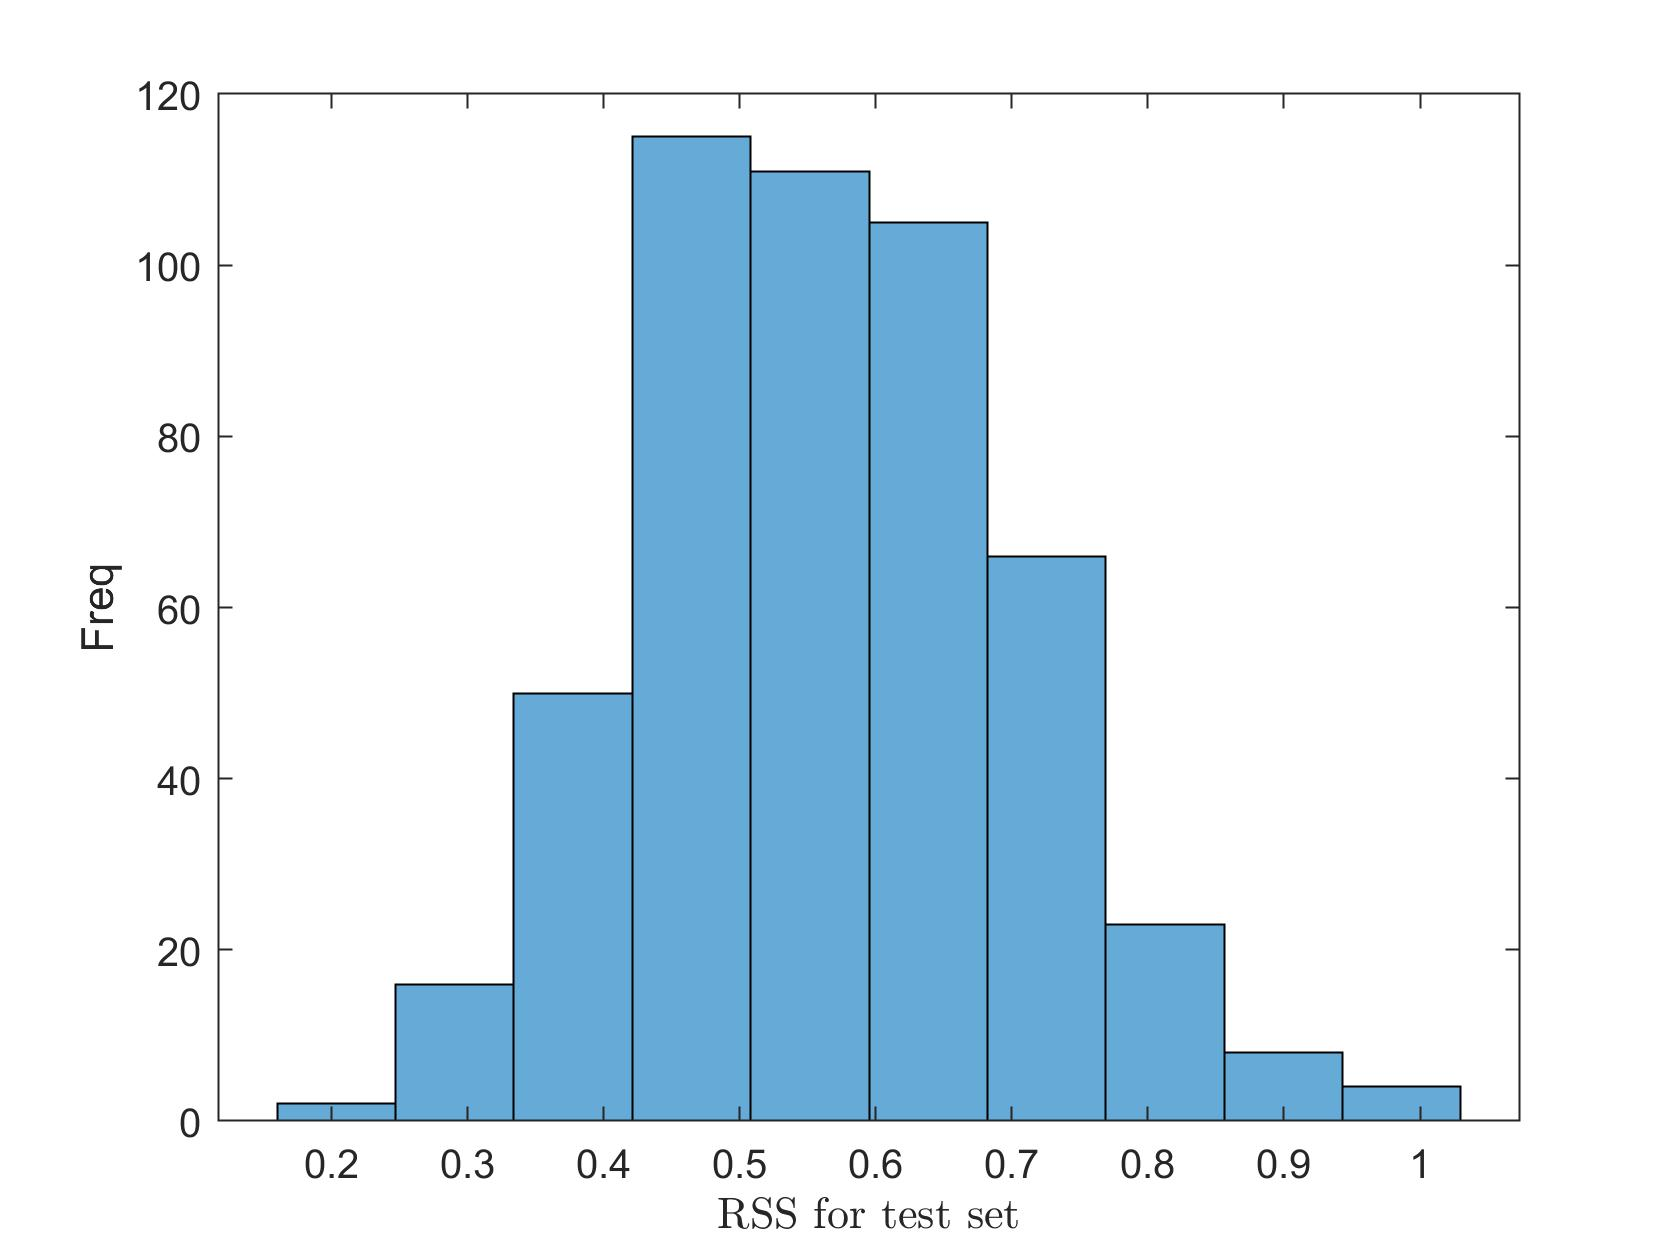
\includegraphics[scale = 0.2]{figures/q8_1_RSStest.jpg}
	\caption{histogram of RSS for test set over 500 repetitions}
	\label{fig:Q8_1_RSStest}
\end{figure}

\begin{figure}[h]
	\centering
	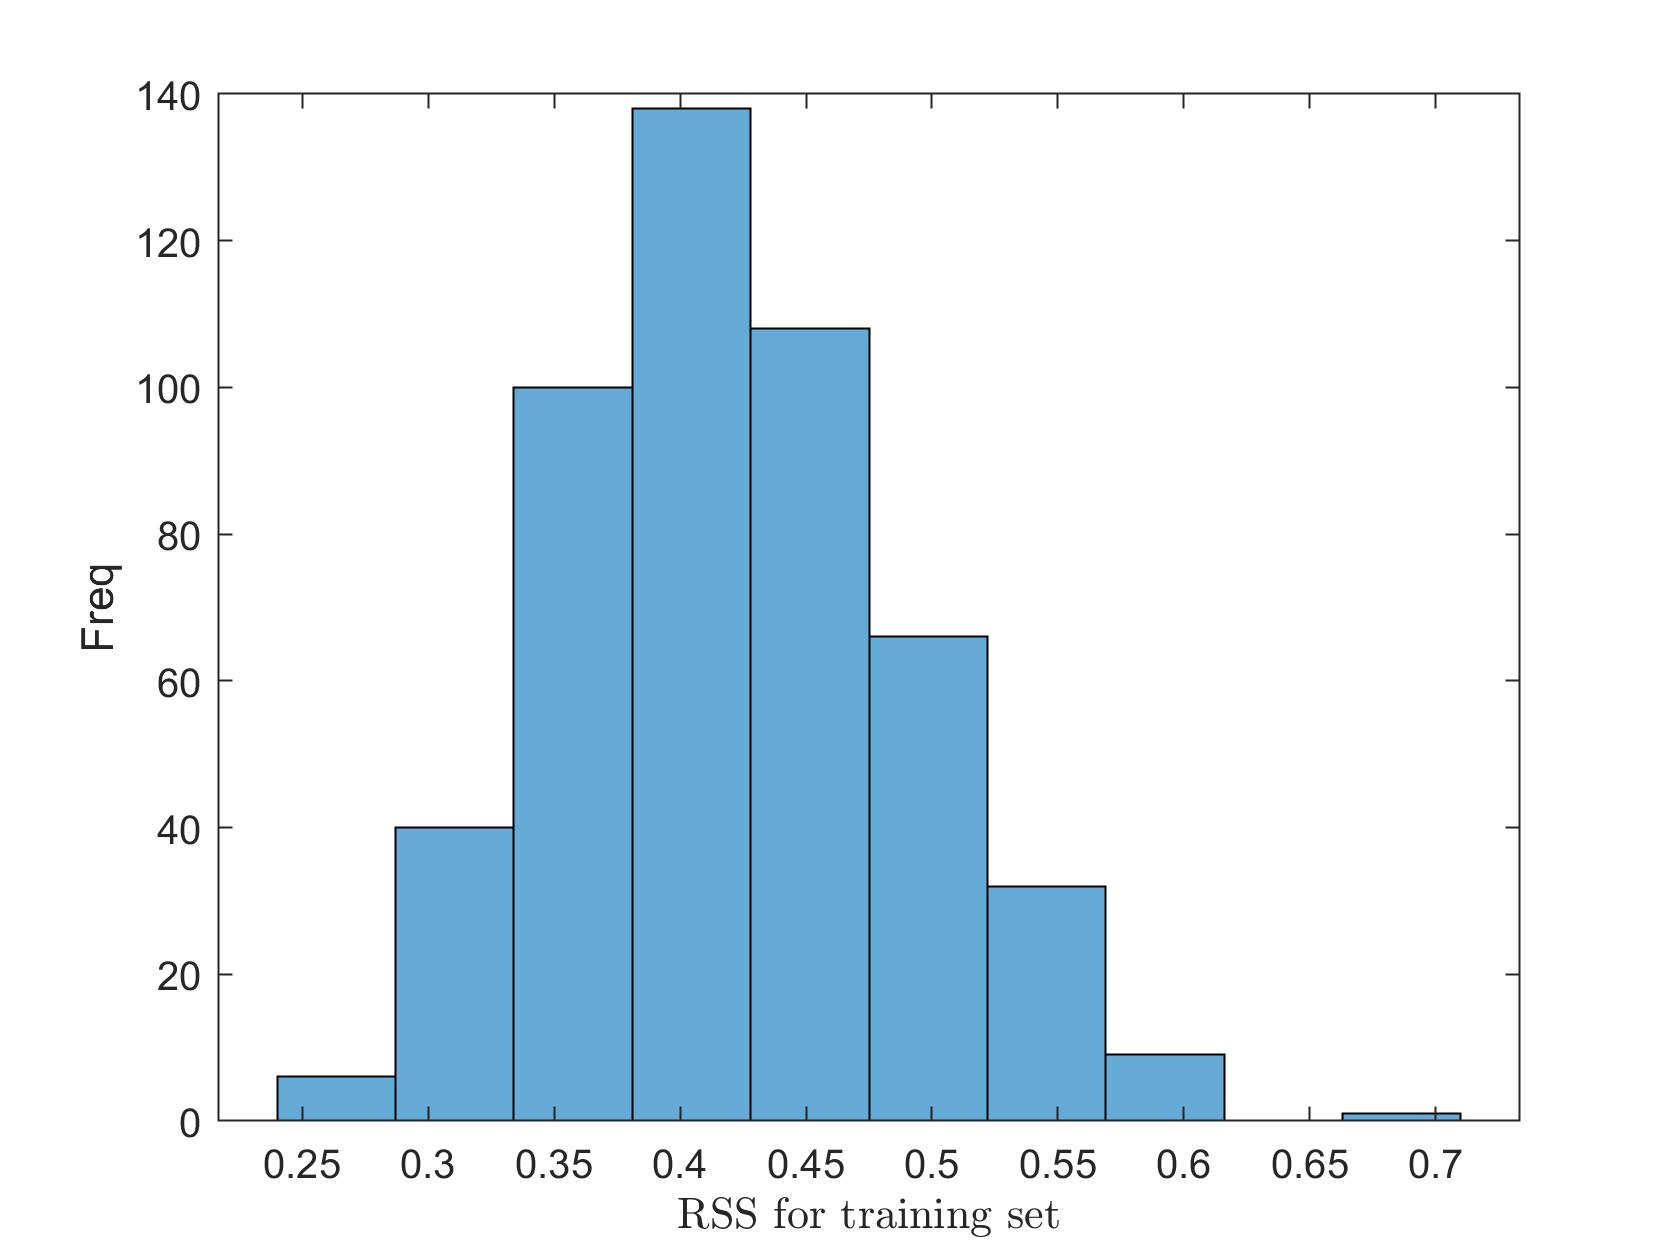
\includegraphics[scale = 0.2]{figures/q8_RSStrain.jpg}
	\caption{histogram of RSS for training set over 500 repetitions}
	\label{fig:Q8_RSStrain}
\end{figure}
	
	\begin{figure}[ht] 
		\begin{subfigure}[b]{0.5\linewidth}
			\centering
			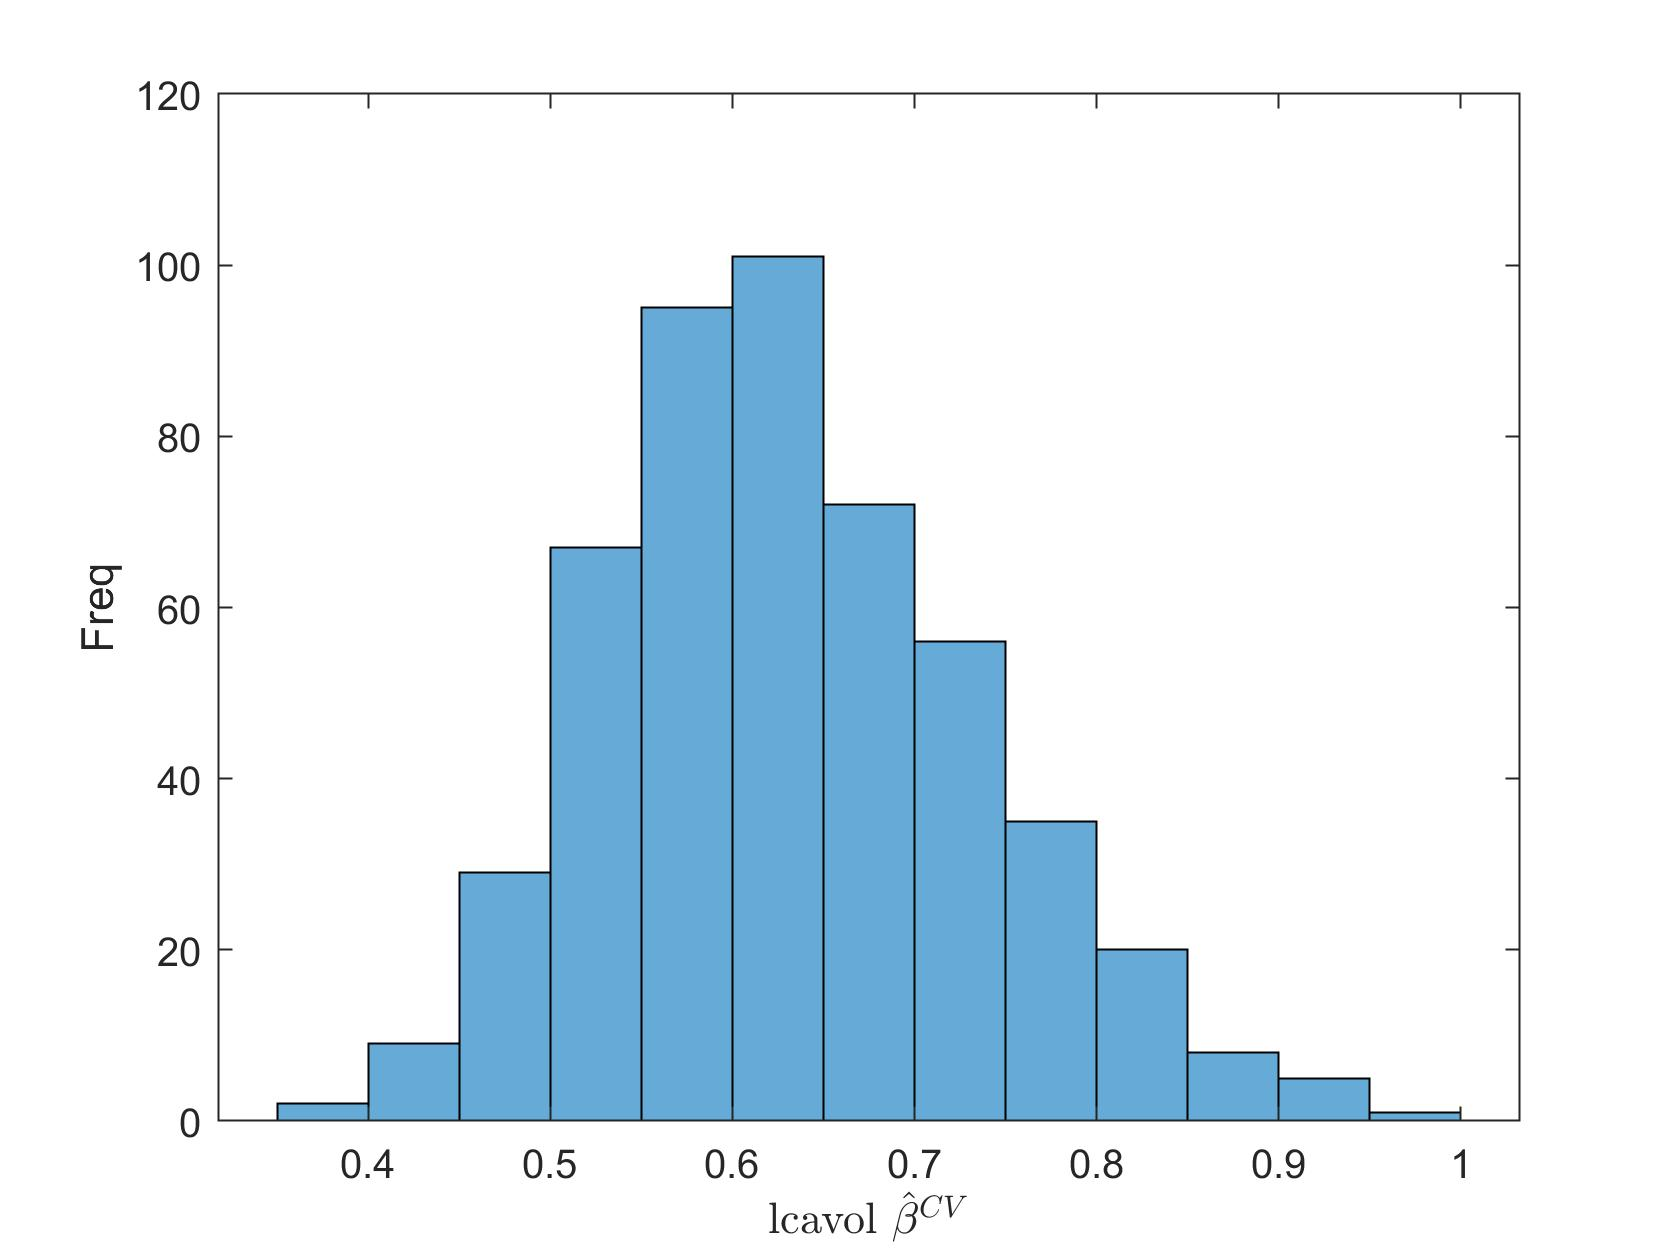
\includegraphics[width=0.75\linewidth]{figures/q8_2.jpg} 
			\caption{lcavol} 
			\label{lcavol} 
			\vspace{4ex}
		\end{subfigure}%% 
		\begin{subfigure}[b]{0.5\linewidth}
			\centering
			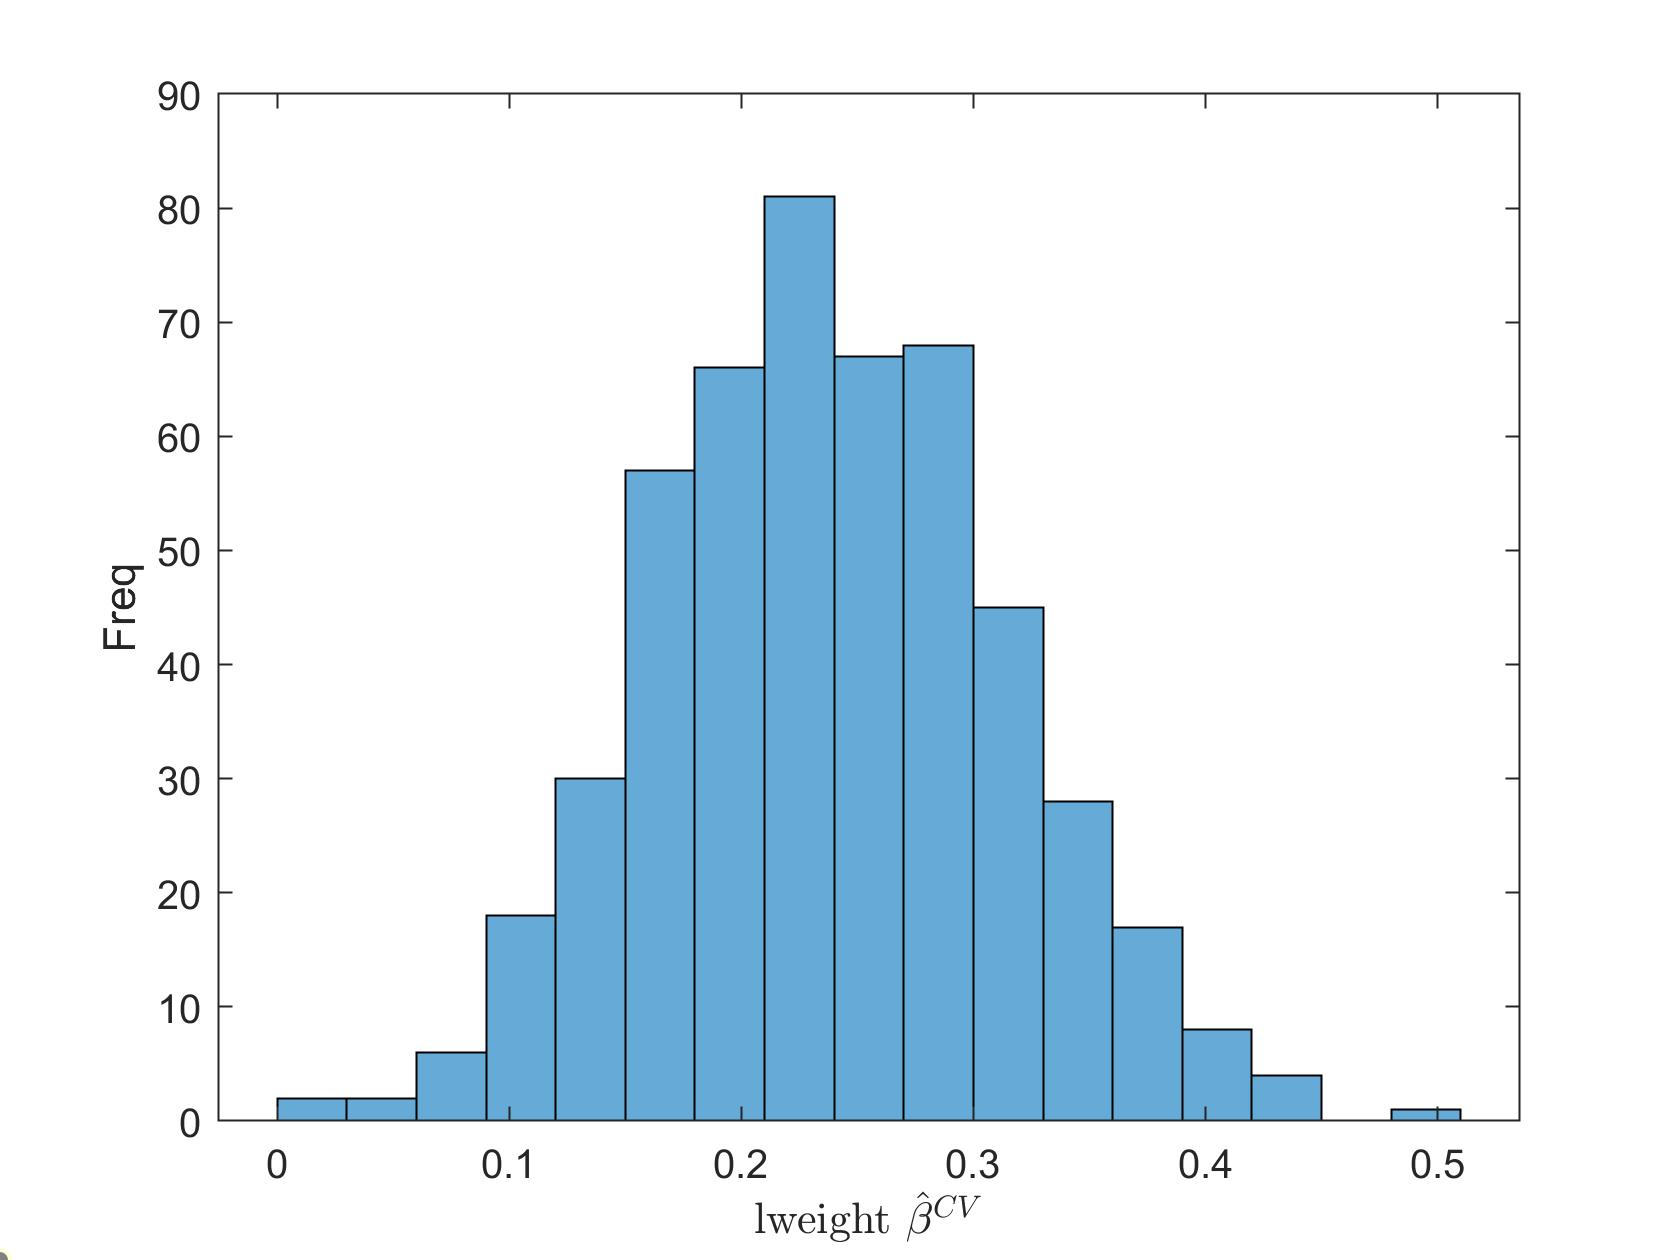
\includegraphics[width=0.75\linewidth]{figures/q8_3.jpg} 
			\caption{lweight} 
			\label{lweight} 
			\vspace{4ex}
		\end{subfigure} 
		\begin{subfigure}[b]{0.5\linewidth}
			\centering
			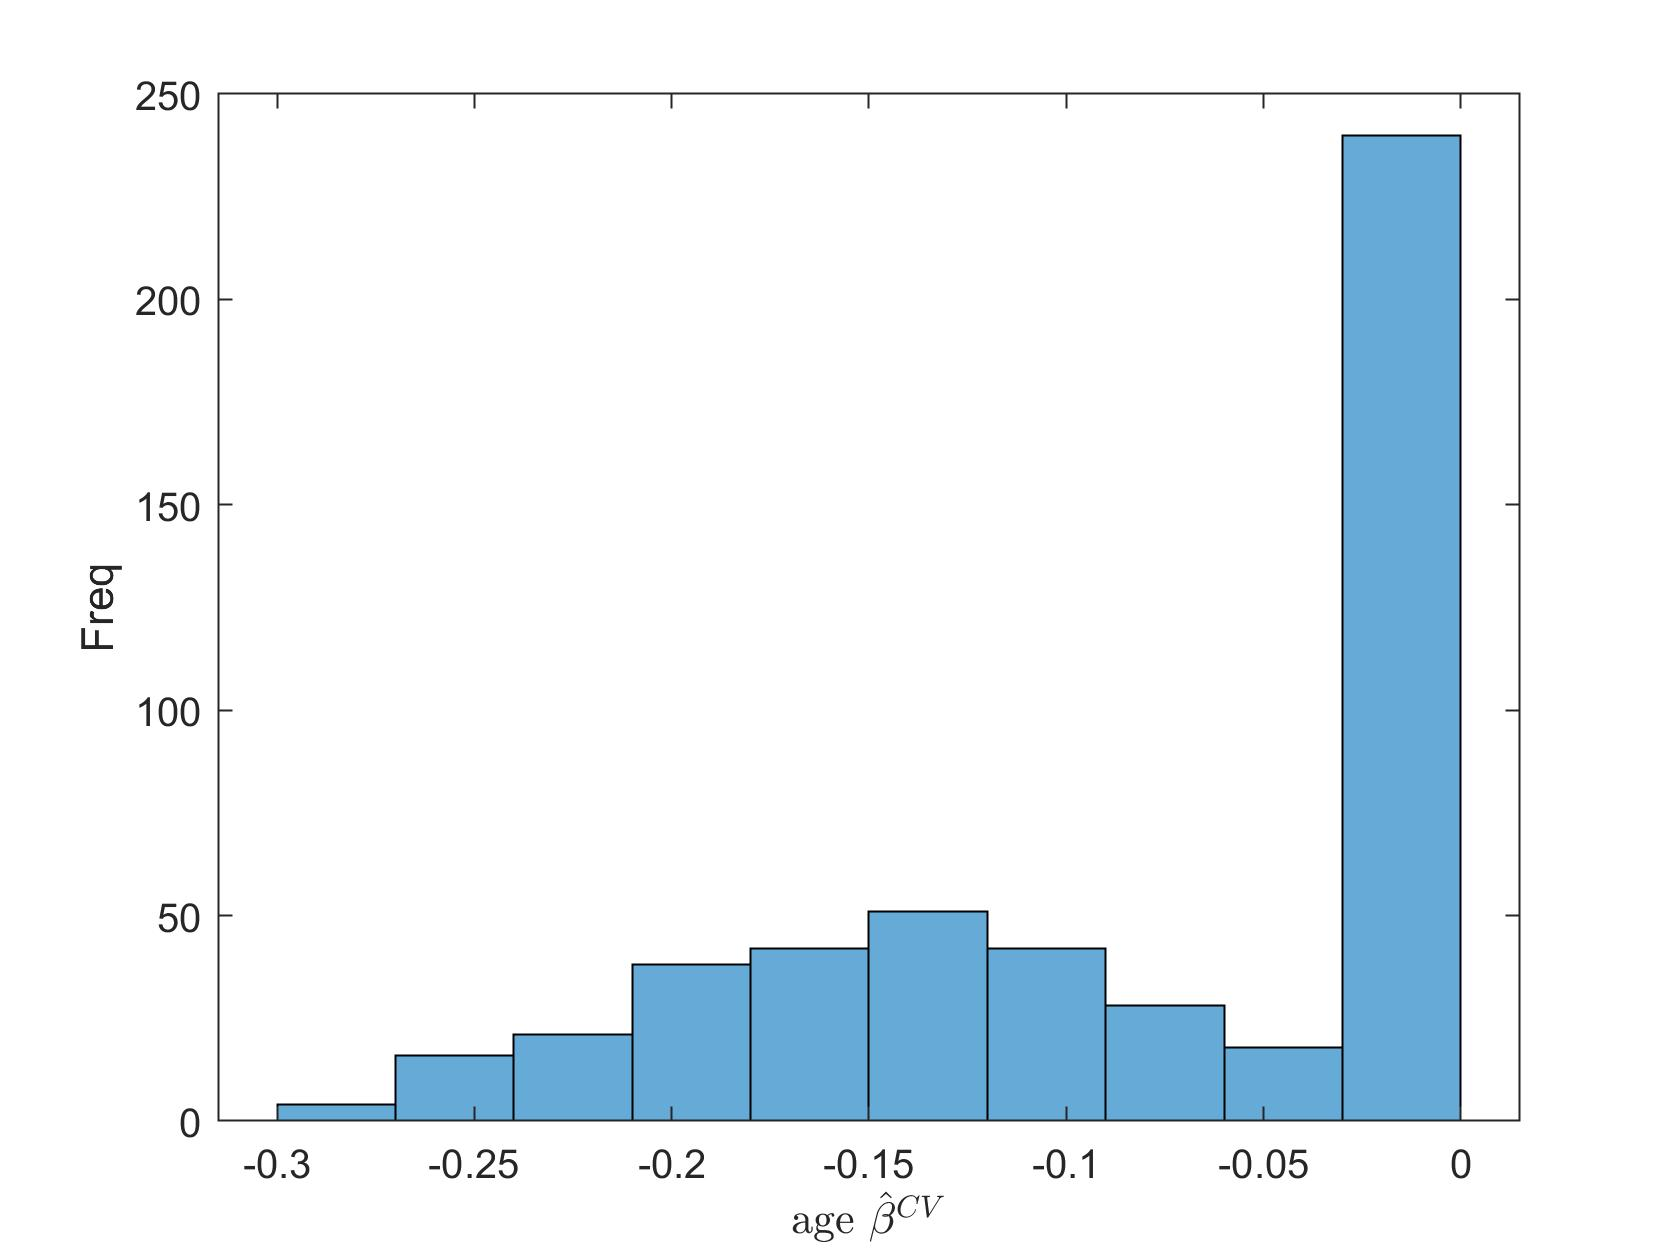
\includegraphics[width=0.75\linewidth]{figures/q8_4.jpg} 
			\caption{age} 
			\label{age} 
		\end{subfigure}%%
		\begin{subfigure}[b]{0.5\linewidth}
			\centering
			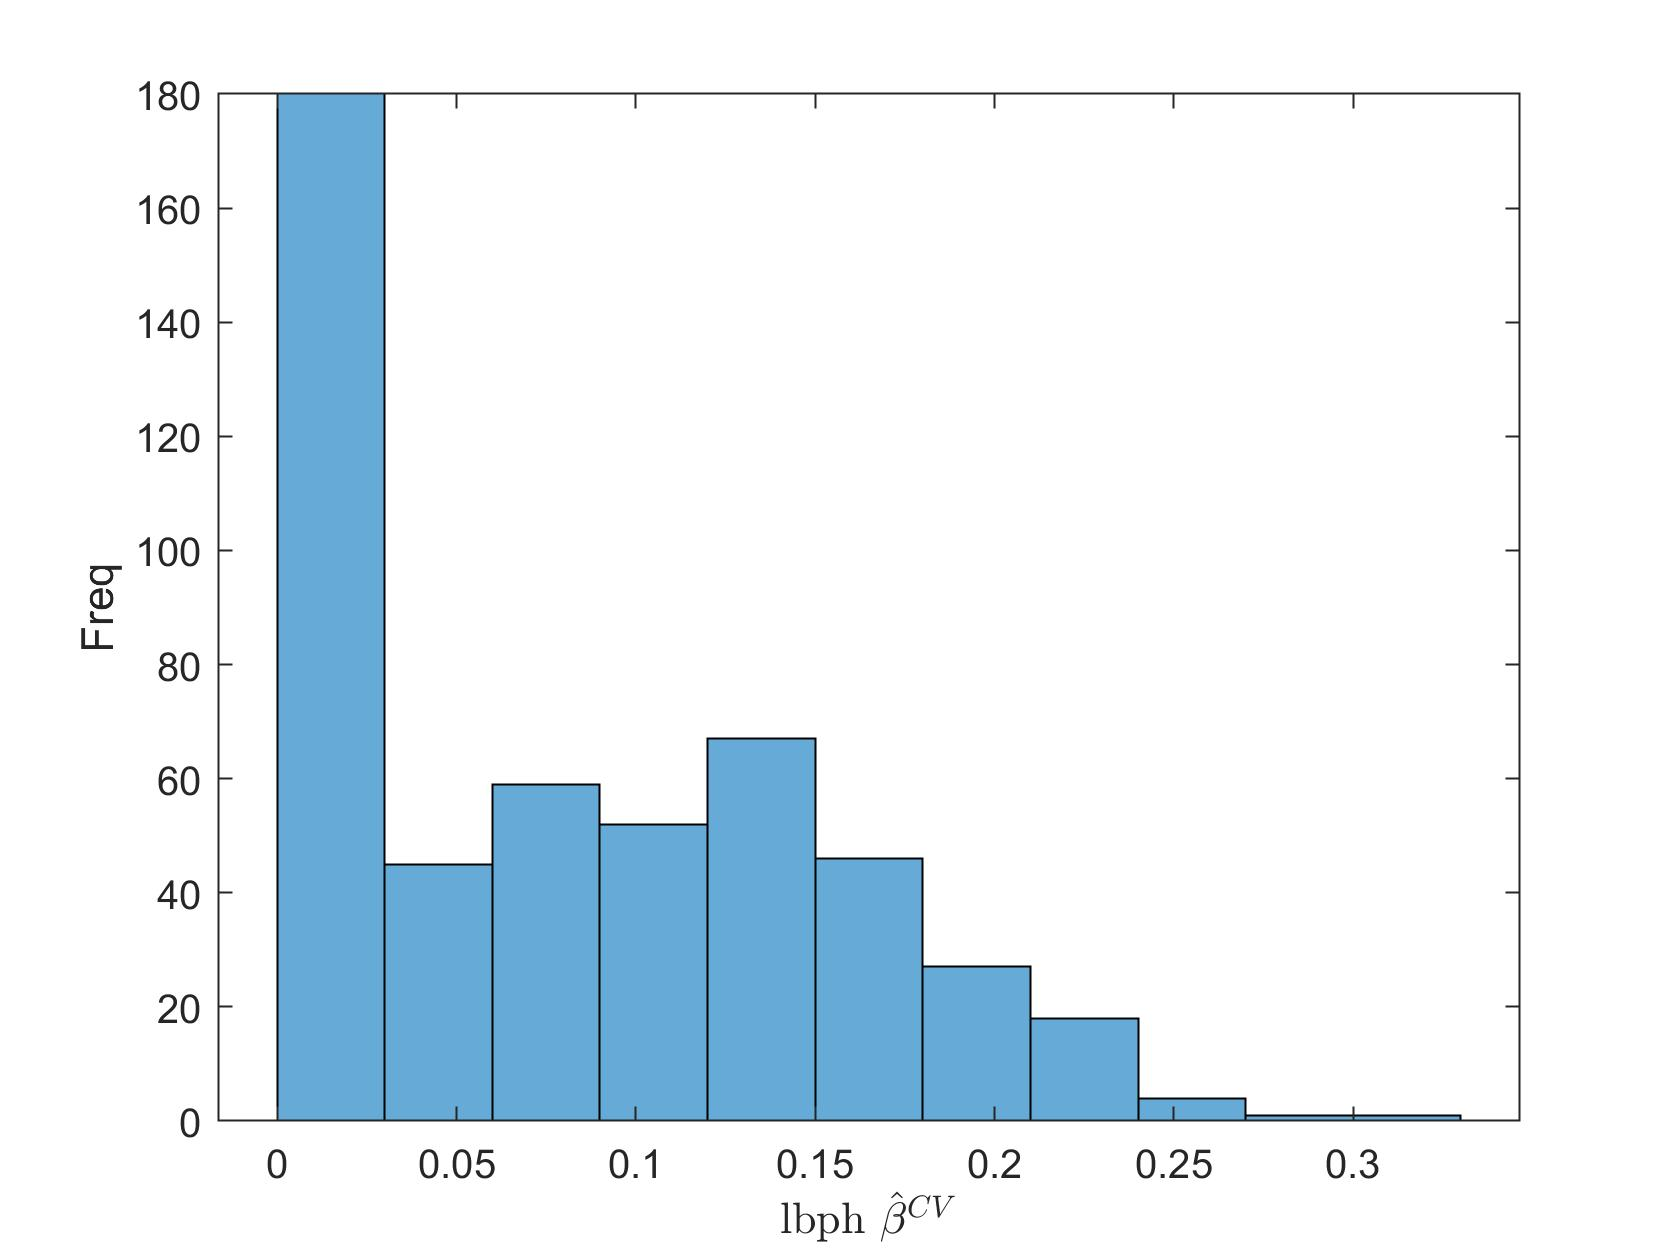
\includegraphics[width=0.75\linewidth]{figures/q8_5.jpg} 
			\caption{lbph} 
			\label{lbph} 
		\end{subfigure} 
		\caption{Histograms corresponding to $ \hat{\beta}^{CV} $ of each covariate over 500 iterations}
		\label{q8_2} 
	\end{figure}

	\begin{figure}[ht] 
		\begin{subfigure}[b]{0.5\linewidth}
			\centering
			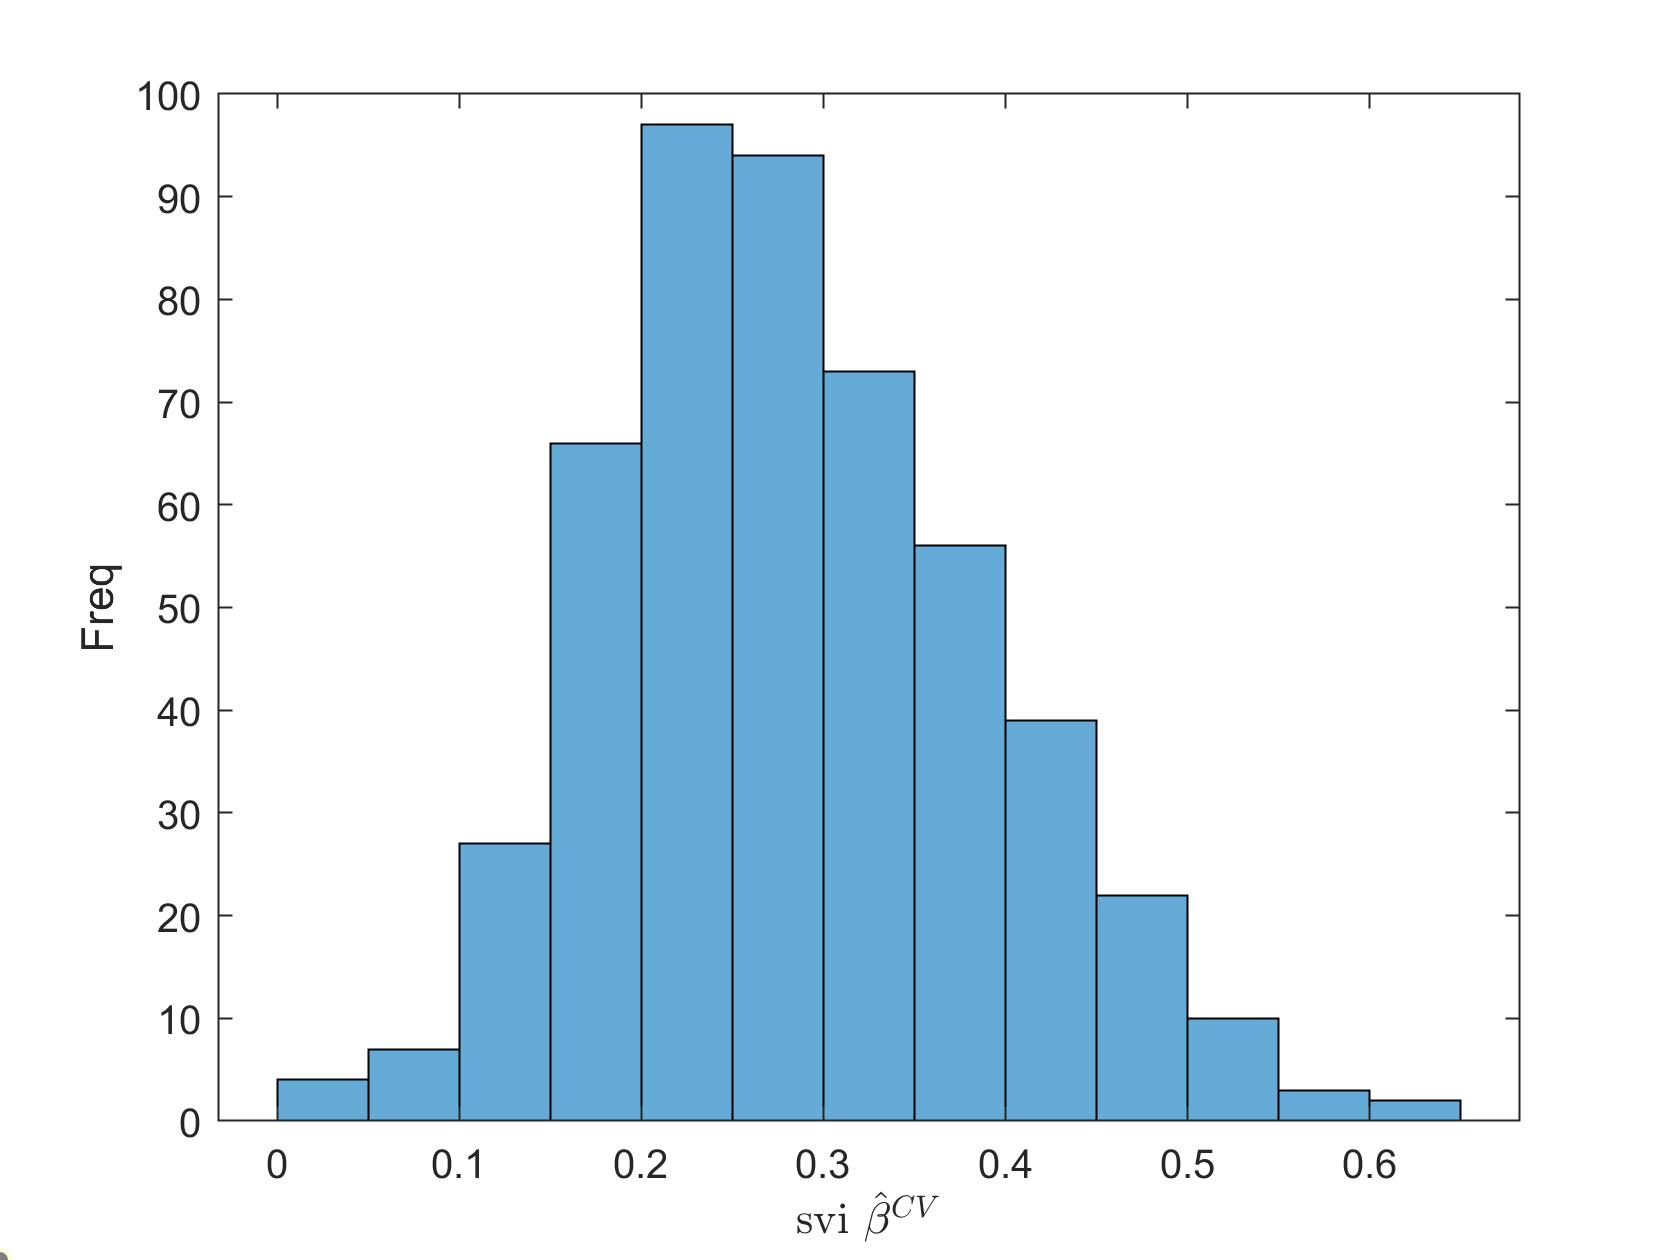
\includegraphics[width=0.75\linewidth]{figures/q8_6.jpg} 
			\caption{svi} 
			\label{svi} 
			\vspace{2ex}
		\end{subfigure}%% 
		\begin{subfigure}[b]{0.5\linewidth}
			\centering
			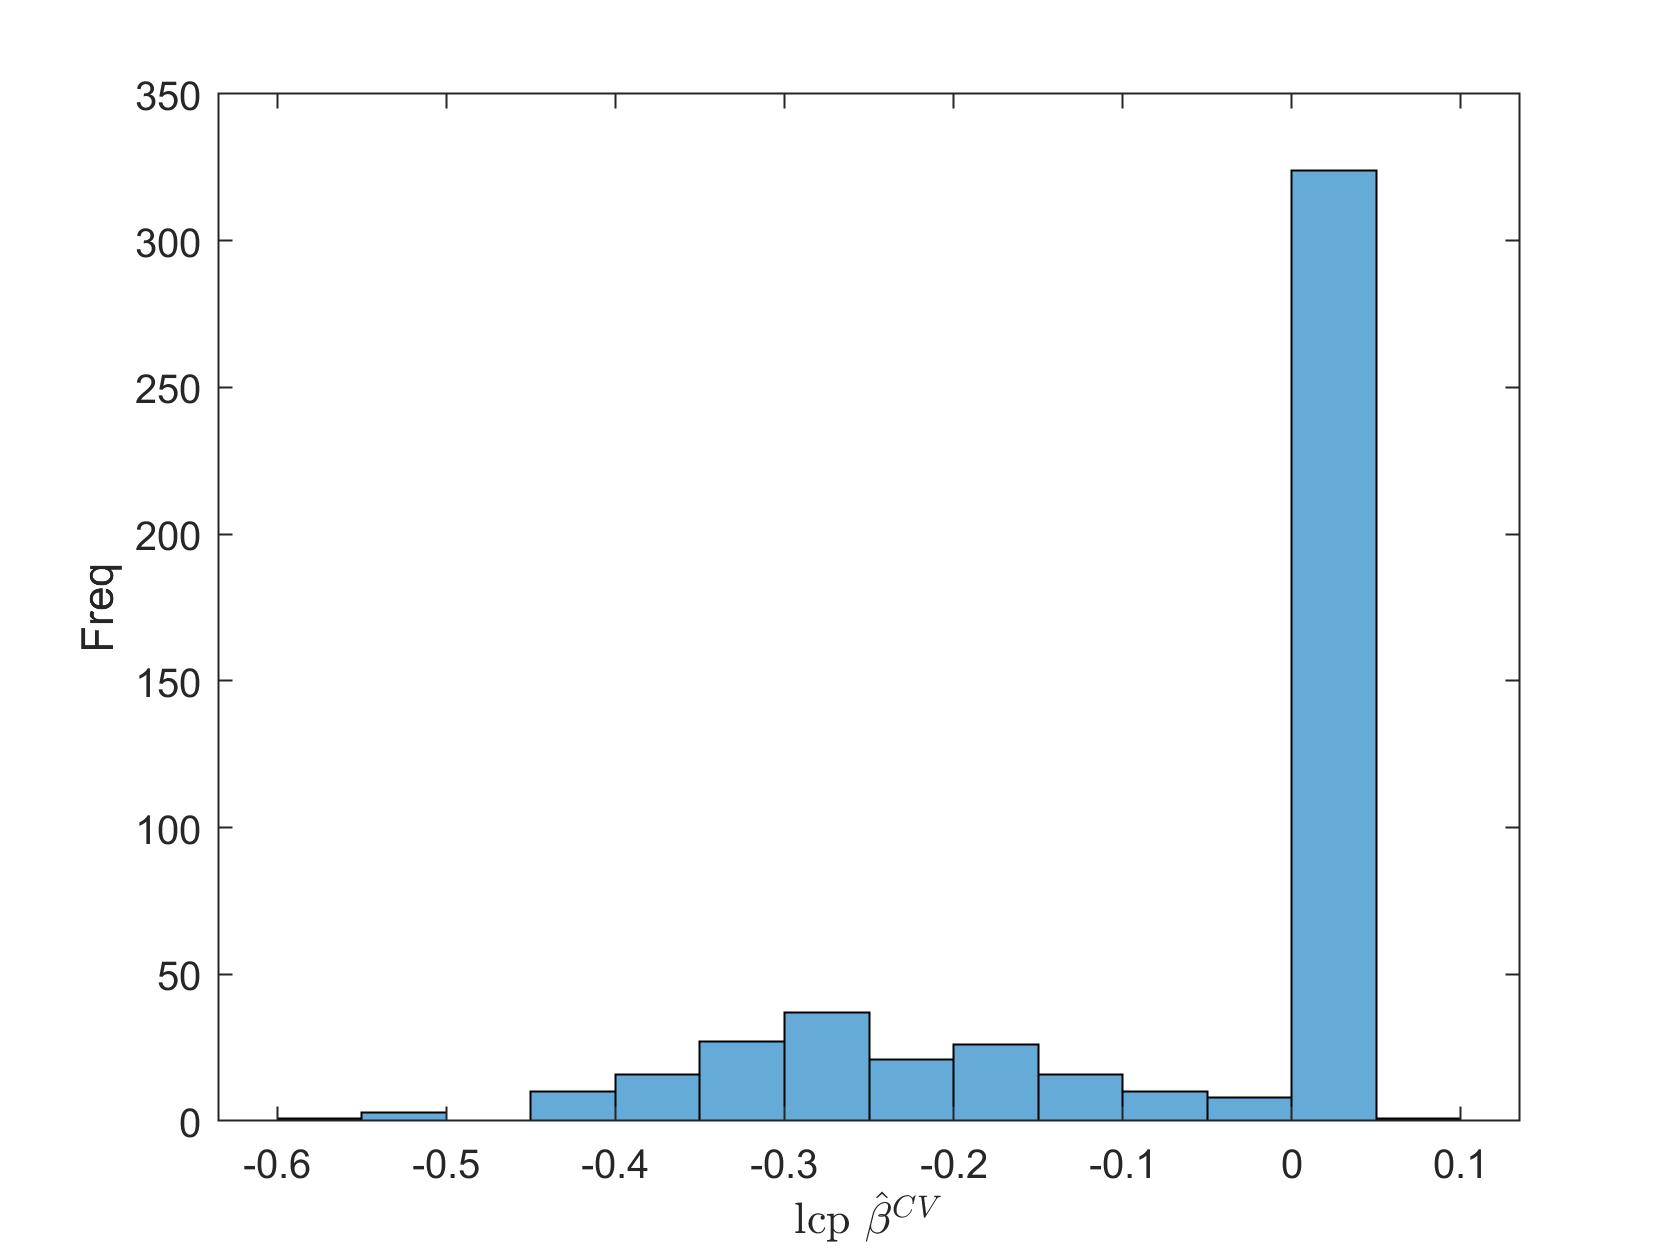
\includegraphics[width=0.75\linewidth]{figures/q8_7.jpg} 
			\caption{lcp} 
			\label{lcp} 
			\vspace{2ex}
		\end{subfigure} 
		\begin{subfigure}[b]{0.5\linewidth}
			\centering
			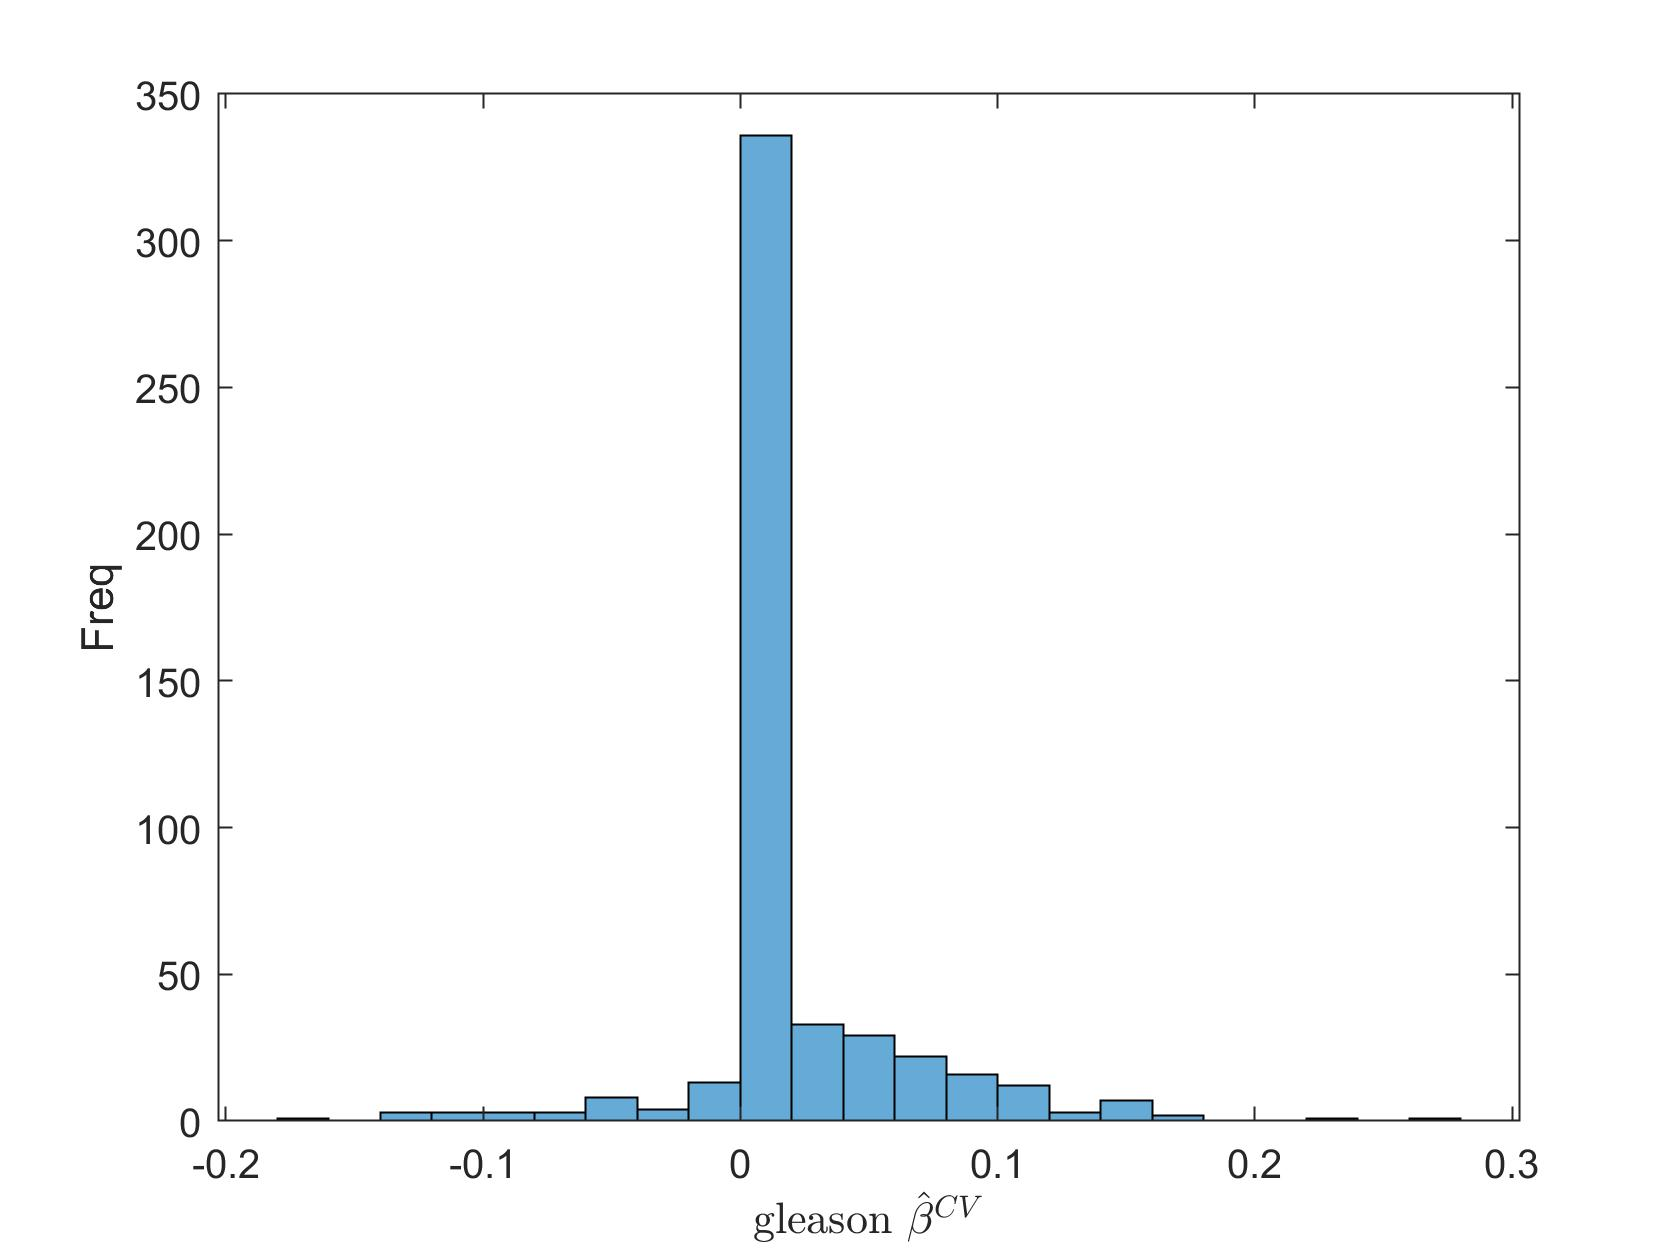
\includegraphics[width=0.75\linewidth]{figures/q8_8.jpg} 
			\caption{gleason} 
			\label{gleason} 
		\end{subfigure}%%
		\begin{subfigure}[b]{0.5\linewidth}
			\centering
			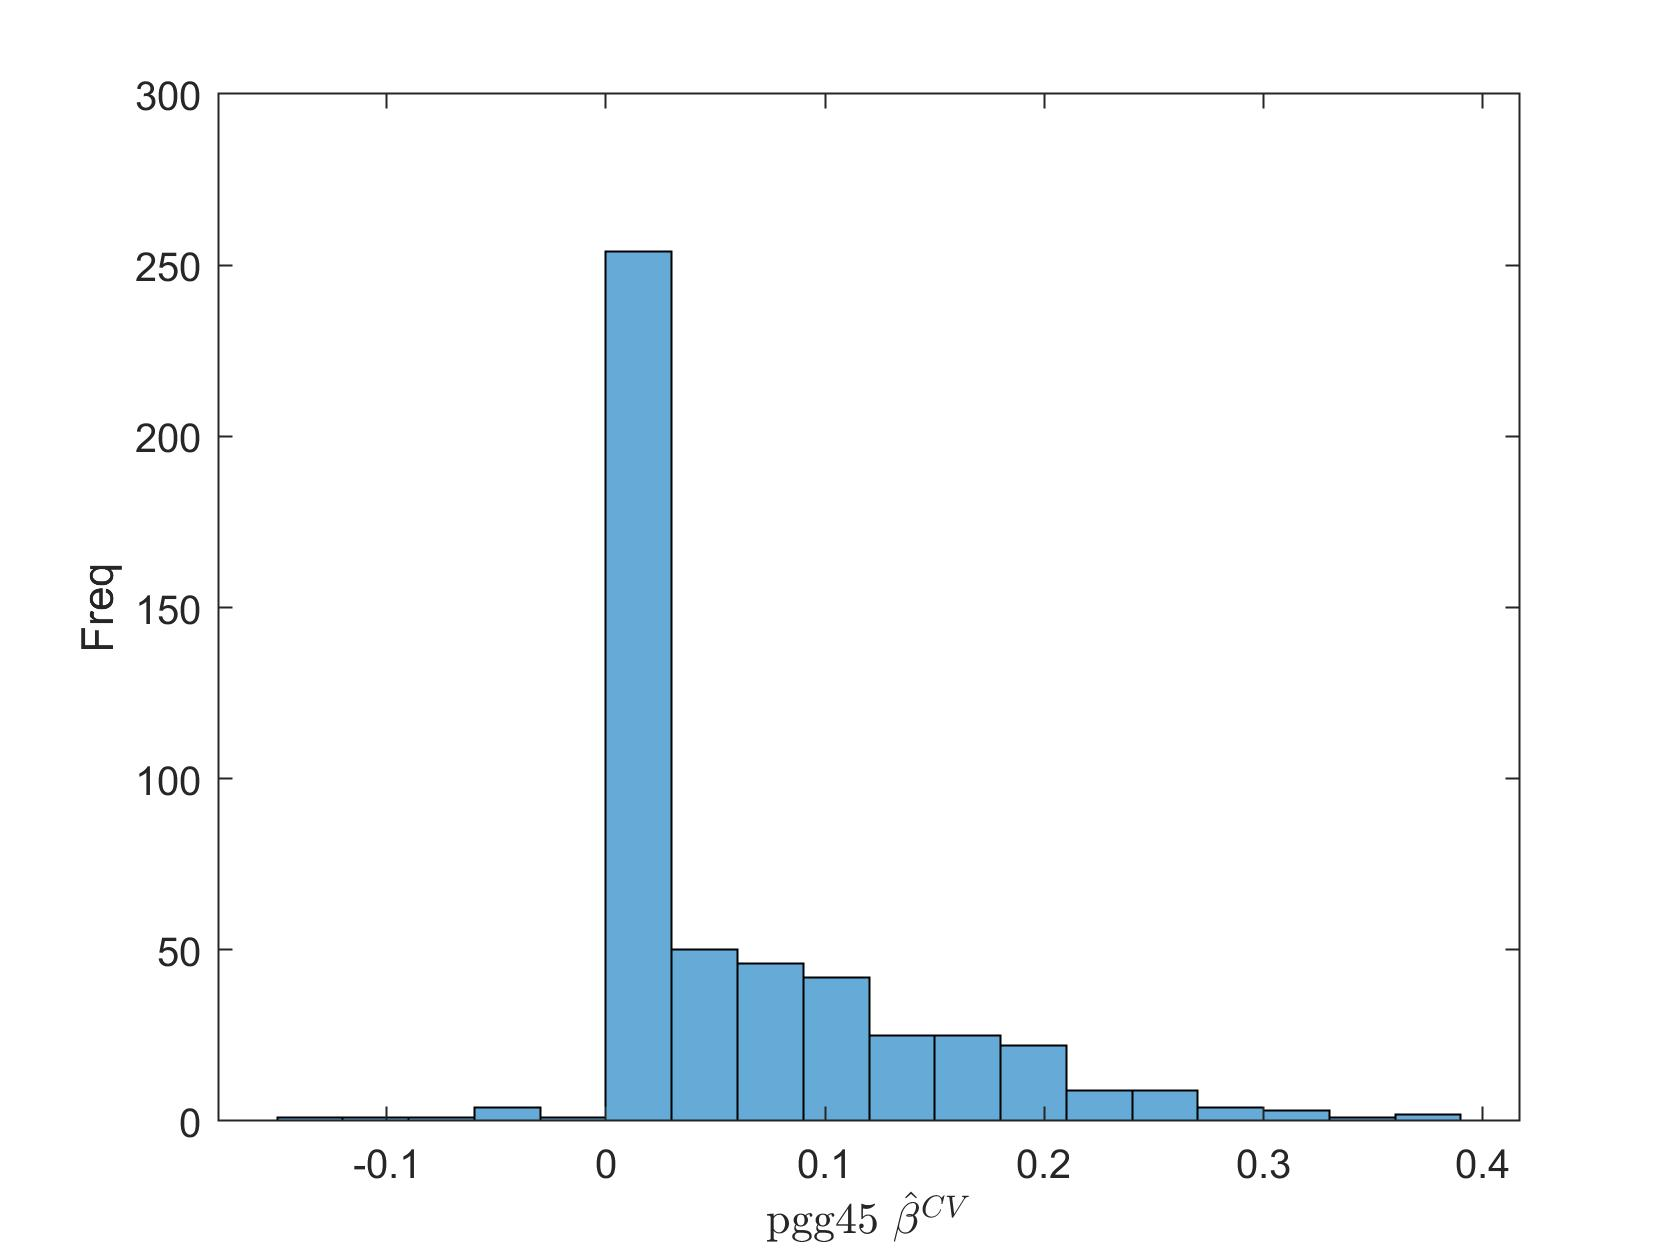
\includegraphics[width=0.75\linewidth]{figures/q8_9.jpg} 
			\caption{pgg45} 
			\label{pgg45} 
		\end{subfigure} 
		\caption{Histograms corresponding to $ \hat{\beta}^{CV} $ of each covariate over 500 iterations}
		\label{q8_3} 
	\end{figure}

\begin{figure}[ht] 
	\begin{subfigure}[b]{0.5\linewidth}
		\centering
		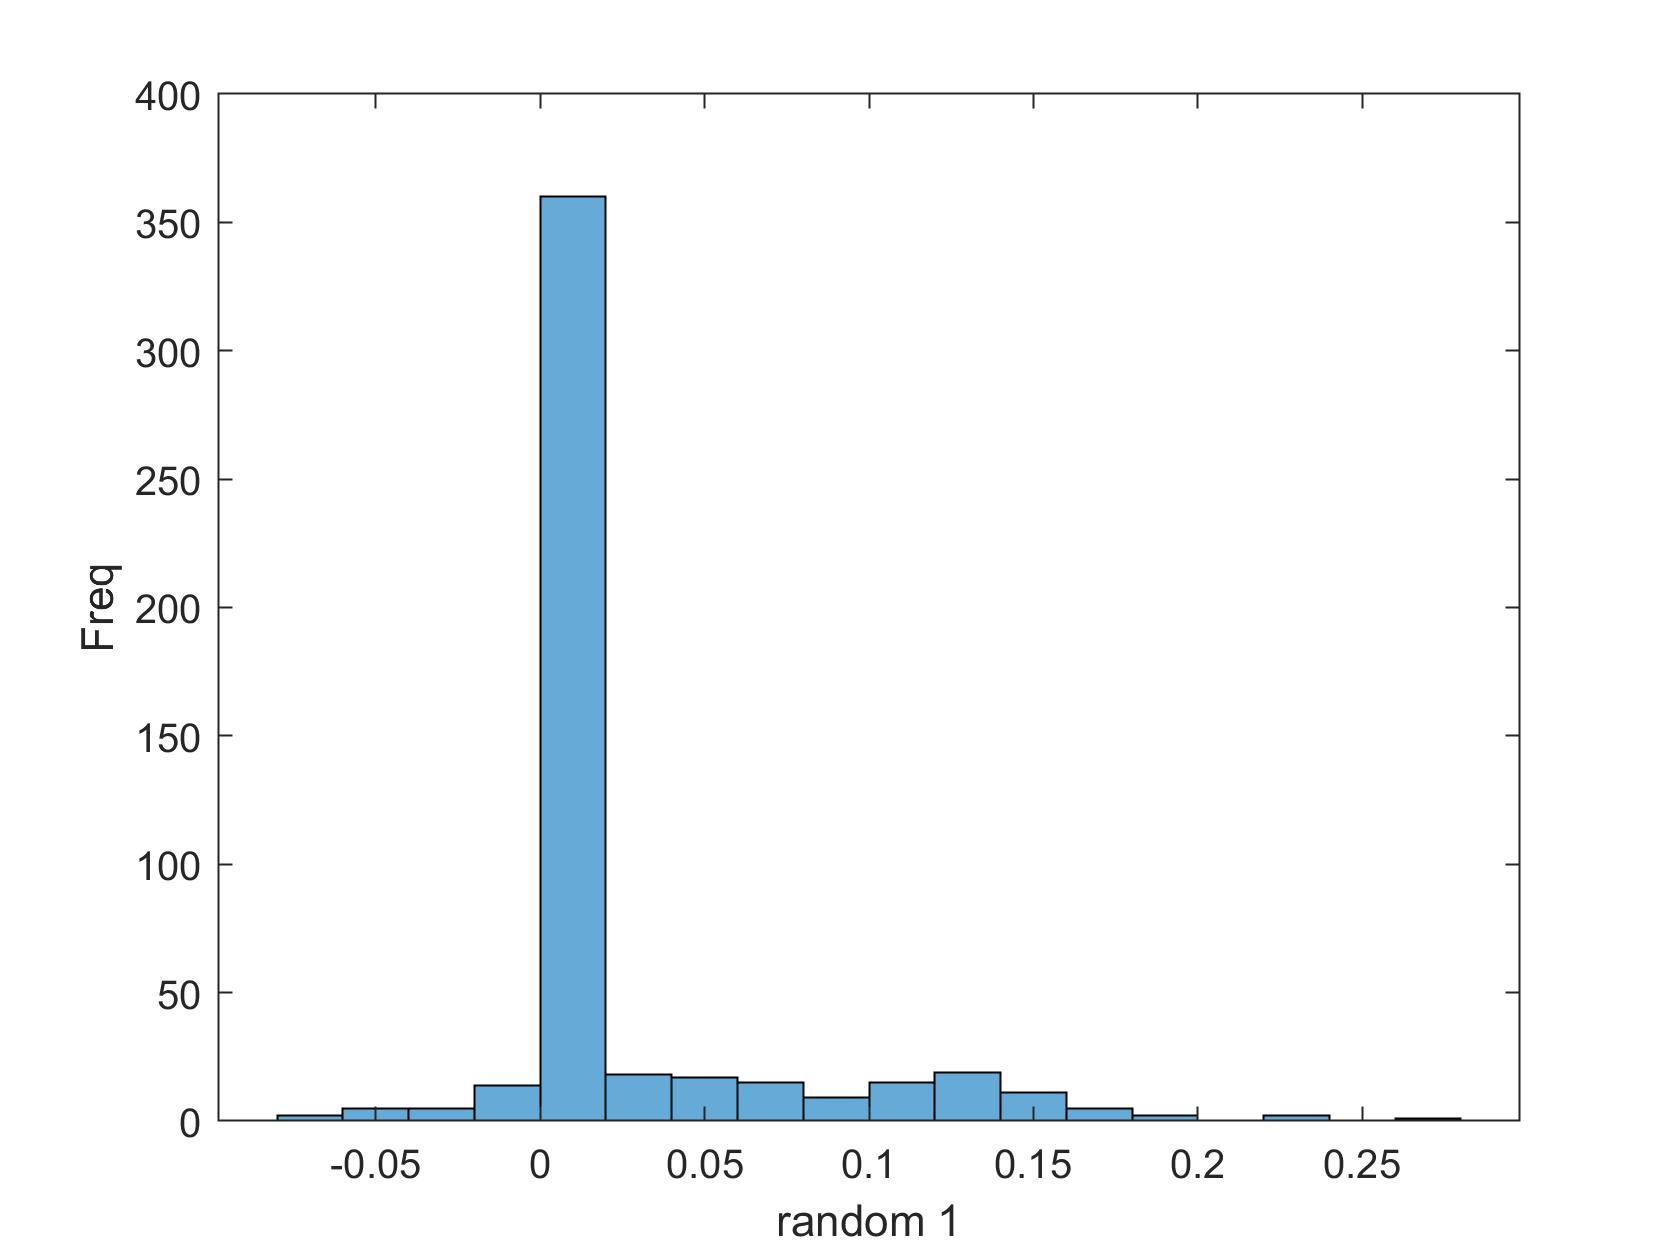
\includegraphics[width=0.75\linewidth]{figures/q8_random1.jpg} 
		\caption{random 1} 
		\label{r1} 
		\vspace{2ex}
	\end{subfigure}%% 
	\begin{subfigure}[b]{0.5\linewidth}
		\centering
		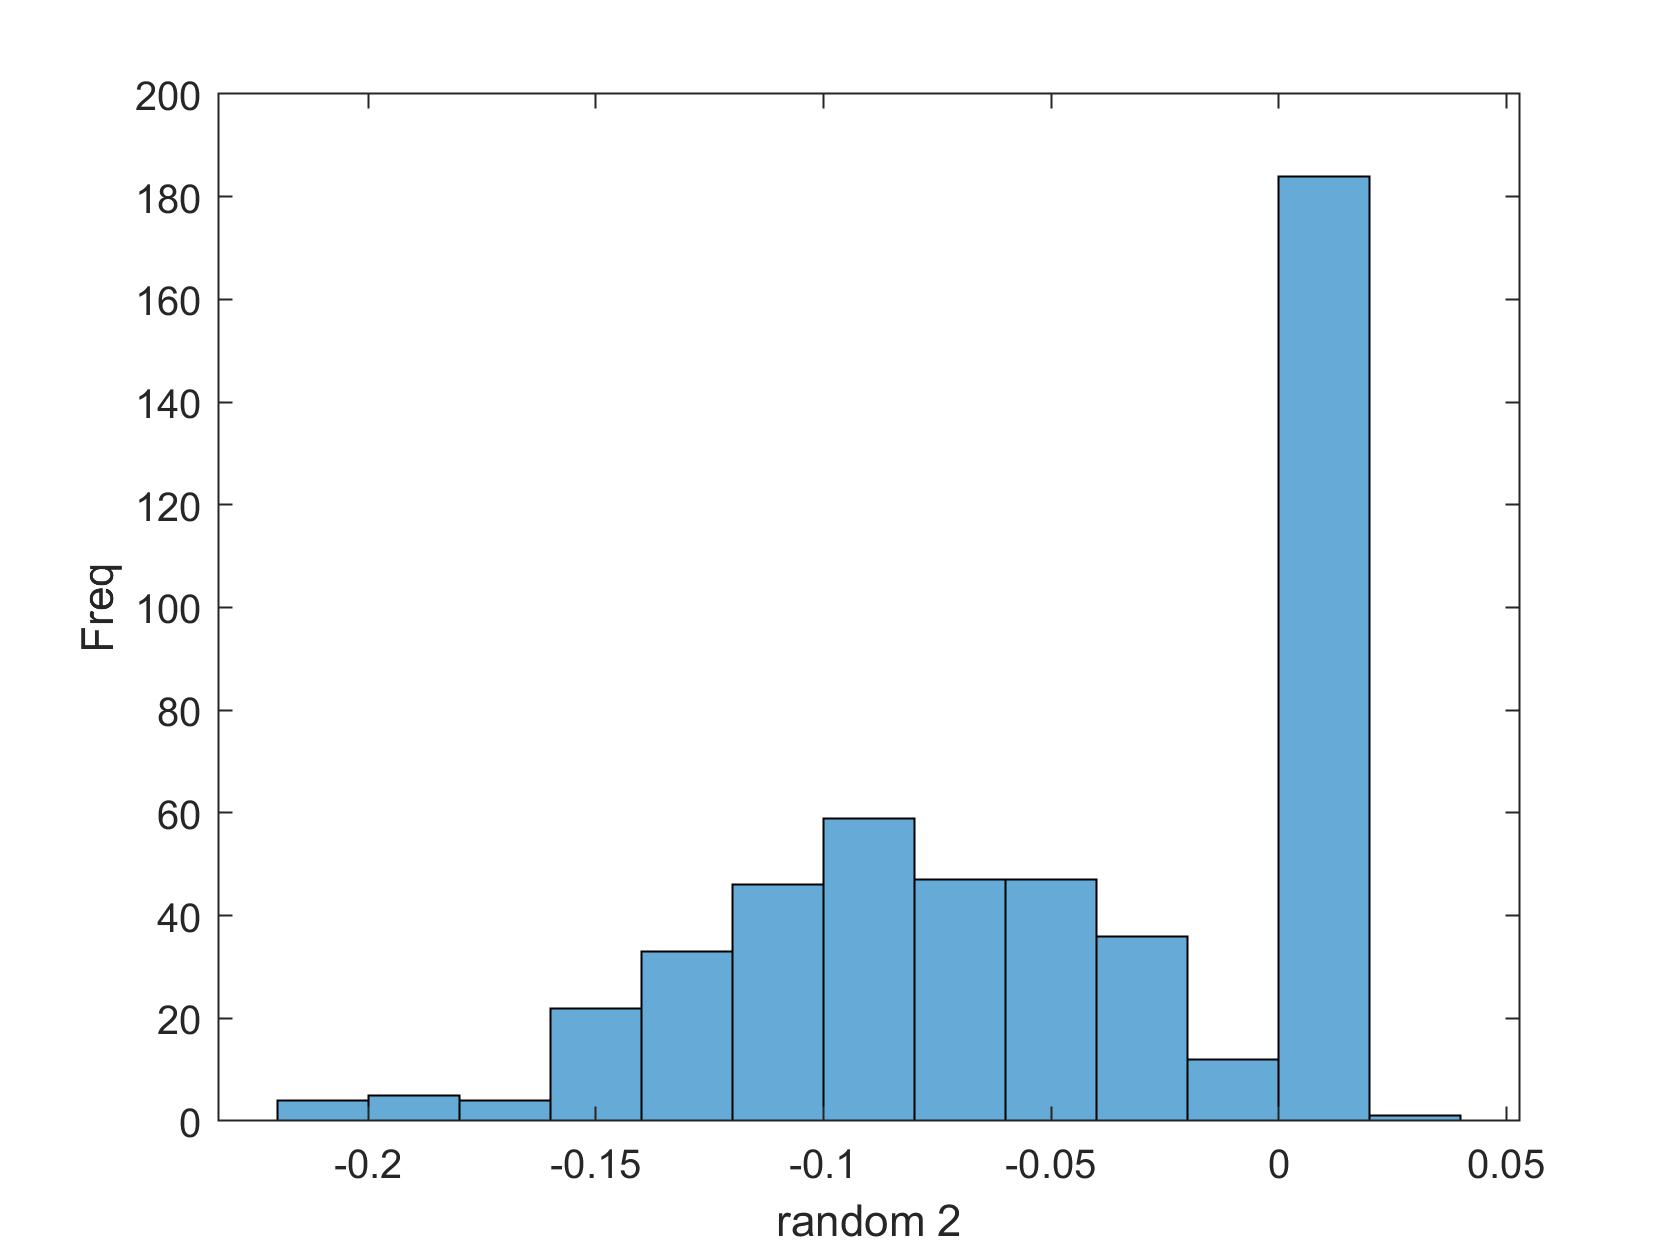
\includegraphics[width=0.75\linewidth]{figures/q8_random2.jpg} 
		\caption{random 2} 
		\label{r2} 
		\vspace{2ex}
	\end{subfigure} 
	\begin{subfigure}[b]{0.5\linewidth}
		\centering
		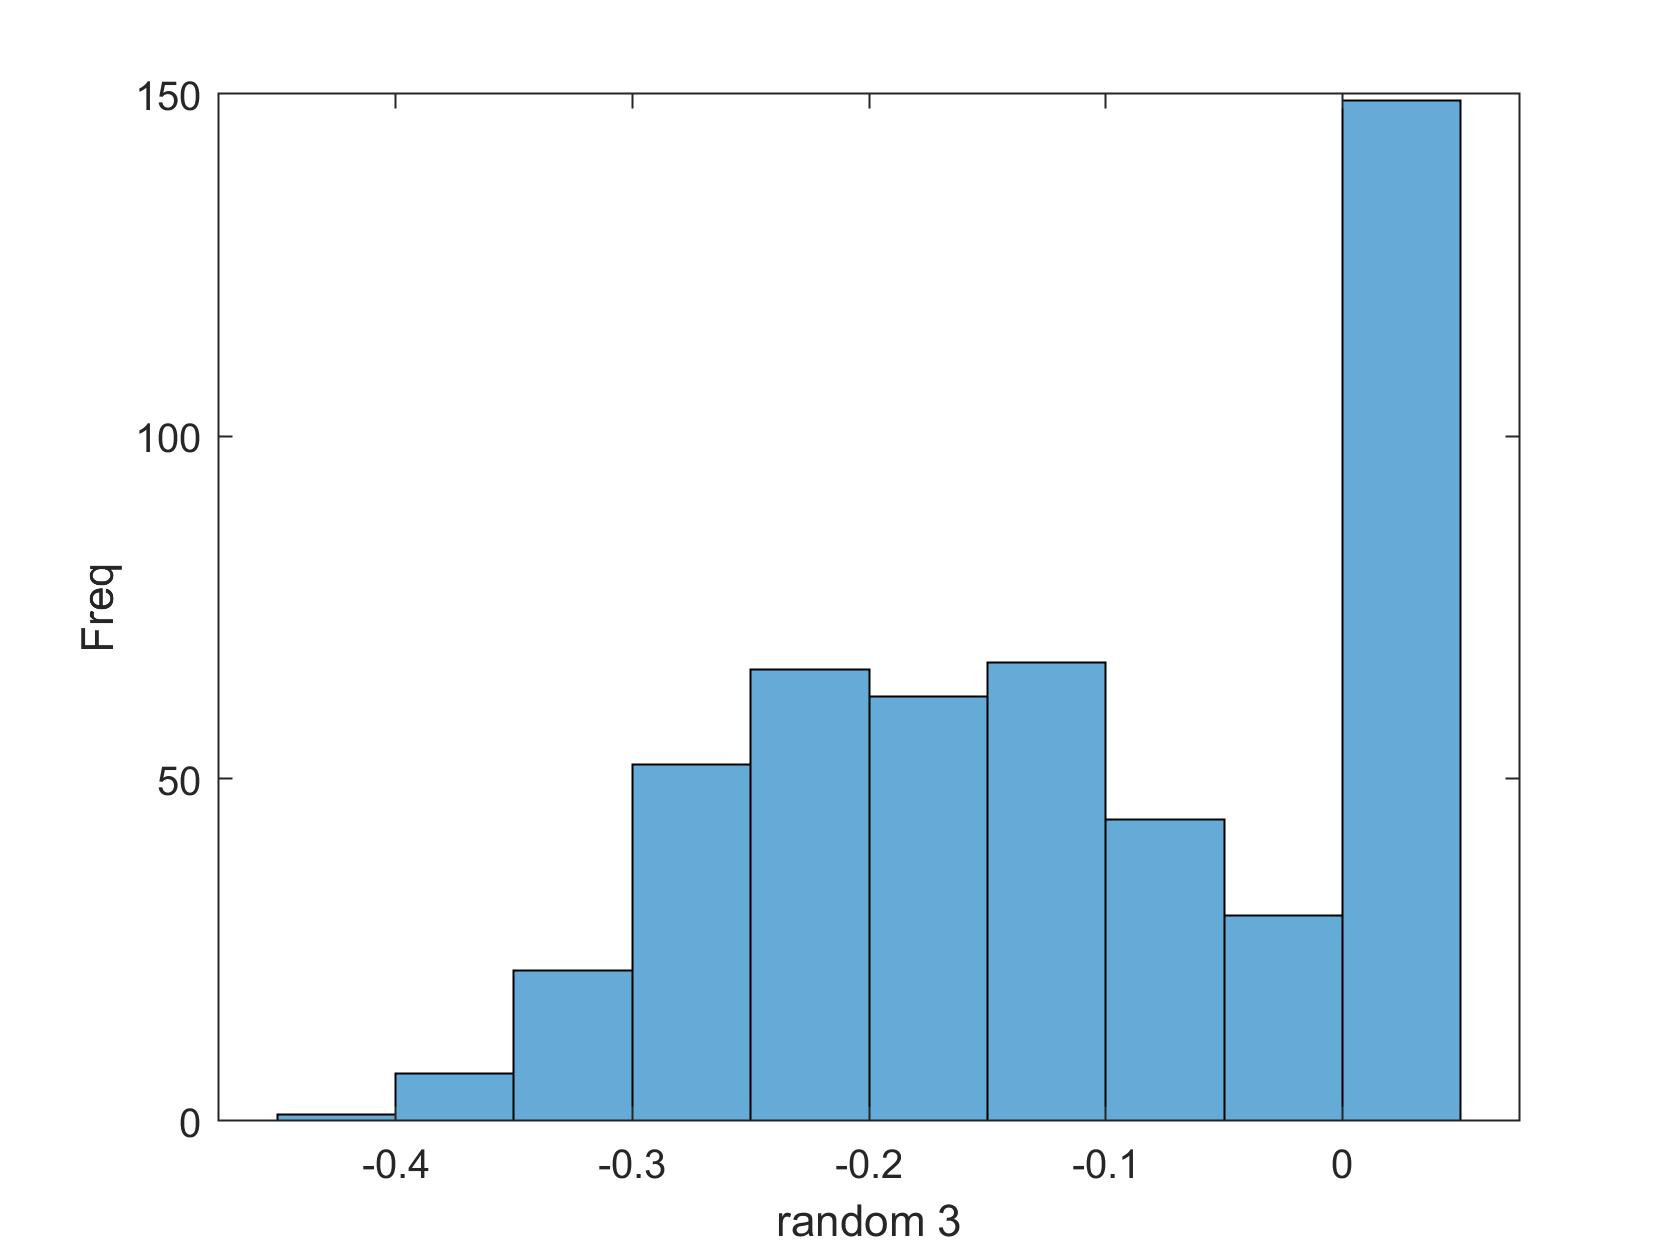
\includegraphics[width=0.75\linewidth]{figures/q8_random3.jpg} 
		\caption{random 3} 
		\label{r3} 
	\end{subfigure}%%
	\begin{subfigure}[b]{0.5\linewidth}
		\centering
		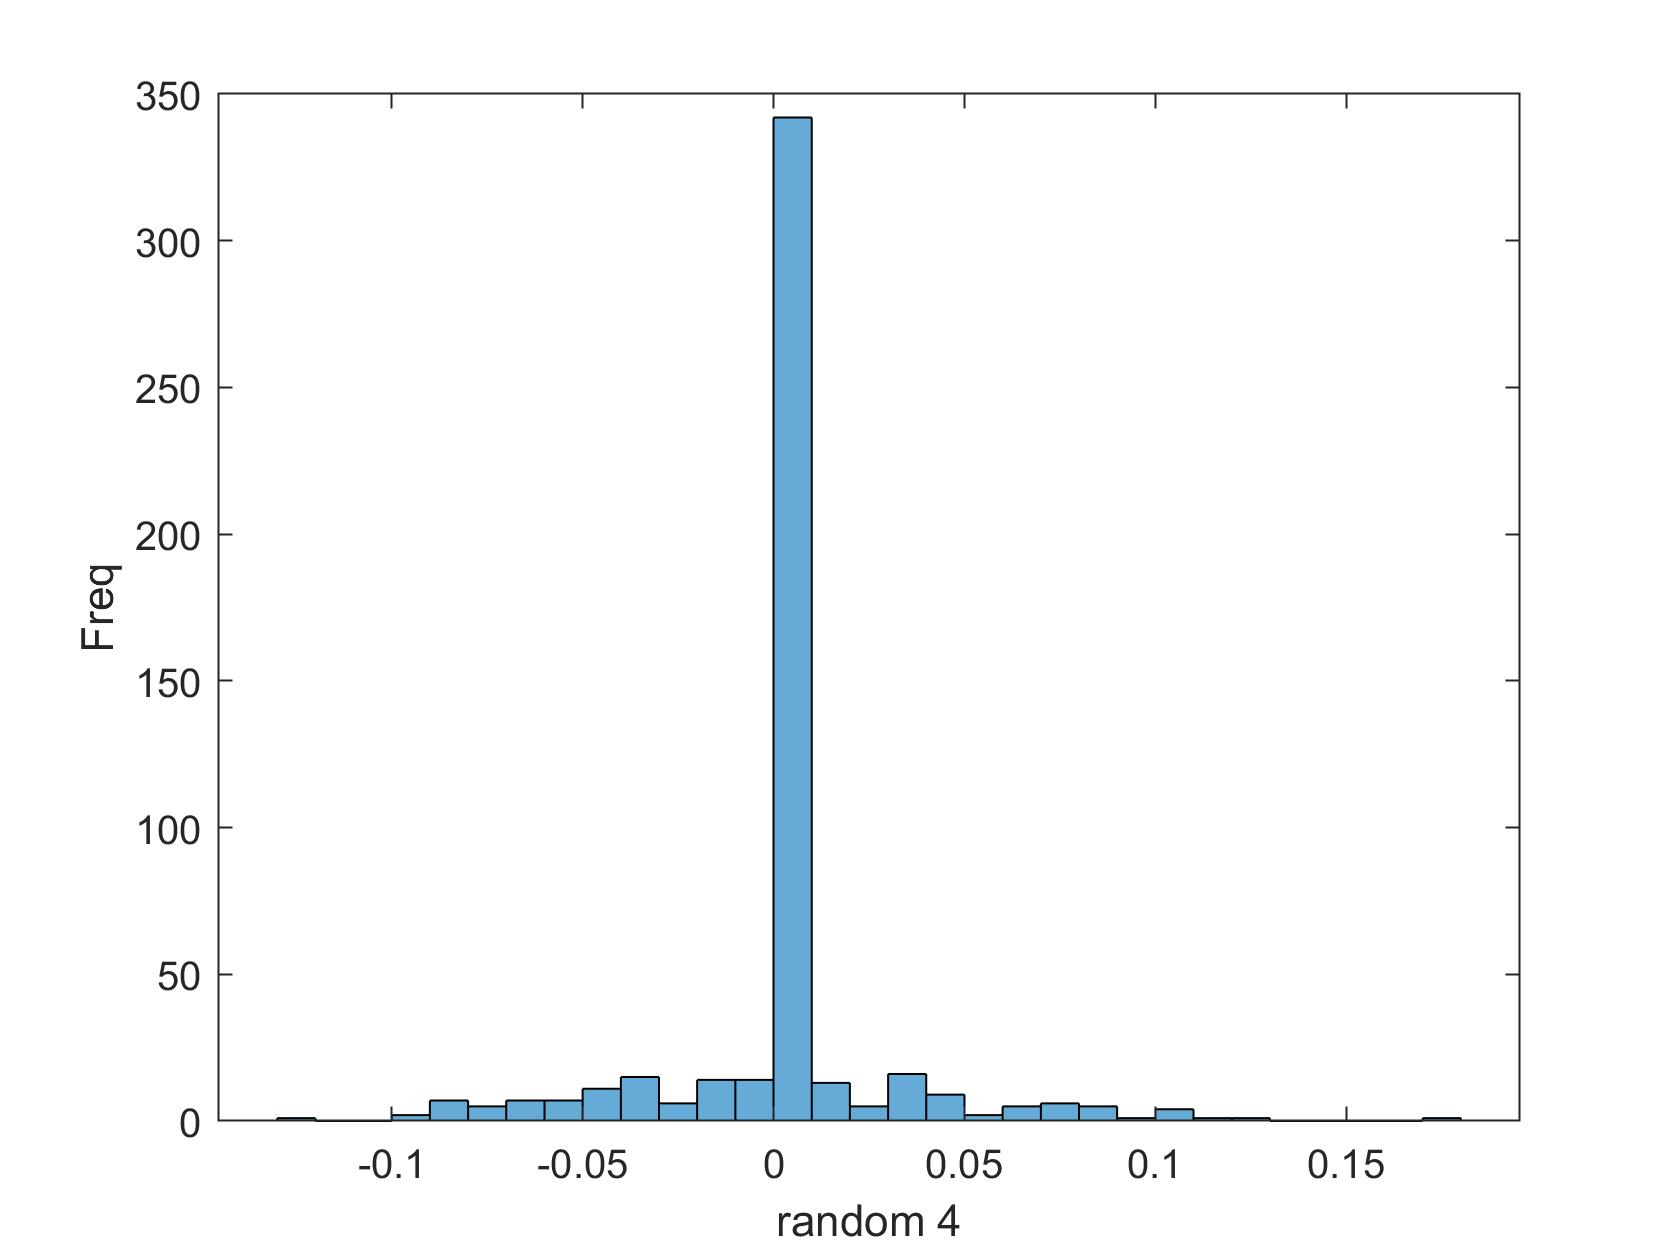
\includegraphics[width=0.75\linewidth]{figures/q8_random4.jpg} 
		\caption{random4} 
		\label{r4}
	\end{subfigure} 
	\caption{Histograms corresponding to $ \hat{\beta}^{CV} $ of each random covariate over 500 iterations}
	\label{q8_4} 
\end{figure}




\clearpage
\newpage
\appendix
\centering\textbf{\huge Appendix}
\section{q2.m}
\label{ap:q2}

\begin{lstlisting}[language = python]
	clear
	format long g
	
	%program files for question 2: q2.m, RSStrte.m
	
	p = 10;
	RSStr_avg = zeros(1, p);
	RSSte_avg = zeros(1, p);
	
	model_size = 1:p;
	
	for i = 1:100
	[RSStr, RSSte] = RSStrte(p);
	RSStr_avg = RSStr_avg + (1/100)*RSStr;
	RSSte_avg = RSSte_avg + (1/100)*RSSte;
	
	end
	
	figure(1)
	hold on;
	scatter(model_size, RSStr_avg);
	scatter(model_size, RSSte_avg);
	l1 = 'RSS training';
	l2 = 'RSS testing';
	xlabel('Model size')
	ylabel('average RSS')
	
	legend(l1, l2)
	
	% %training size Ntr = 30
	% title('RSS when training set has size 30')
	% exportgraphics(gcf,'q2_1.jpg','Resolution',300)
	
	%when Ntr = 200
	title('RSS when training set has size 200')
	exportgraphics(gcf,'q2_2.jpg','Resolution',300)
\end{lstlisting}

\section{RSStrte.m}
\label{ap:RSStrte}
\begin{lstlisting}[language = python]
	function [RSStr, RSSte] = RSStrte(p)
	Ntr = 200;
	Nte = 1000;
	
	
	%training:
	Xtr = normrnd(0, 1, Ntr, p);
	Xte = normrnd(0, 1, Nte, p);
	
	Etr = normrnd(0, 1, Ntr, 1);
	Ete = normrnd(0, 1, Nte, 1);
	
	beta = [-0.5 -0.45 -0.4 0.35 -0.3 0.25 -0.2 0.15 -0.1 0.05]';
	
	Ytr = Xtr*beta + Etr;
	Yte = Xte*beta + Ete;
	
	RSStr = zeros(1, p);
	RSSte = zeros(1, p);
	
	for j = 1:p 
	
	XM = Xtr(:, [1:j]);
	betaM = inv(XM' * XM) * XM' * Ytr;
	%find training error
	for i = 1:Ntr
	
	RSStr(j) = RSStr(j) + (1/Ntr)*(Ytr(i) - XM(i, :)*betaM).^2;
	end
	
	XMte = Xte(:, [1:j]);
	%now for test error
	for k = 1:Nte
	RSSte(j) = RSSte(j) + (1/Nte)*(Yte(k) - XMte(k, :)*betaM).^2;
	end
	end
\end{lstlisting}

\section{q3.m}
\label{ap:q3}
\begin{lstlisting}[language= python]
	clear
	format long g
	
	%for this question the relevant program files are q3.m, bestsubset.m and
	%generateTrain.m
	
	p = 10;
	N = 30;
	T = generateTrain(p, N);
	
	B = bestsubset(T);
\end{lstlisting}

\section{bestsubset.m}
\label{ap:bestsubset}
\begin{lstlisting}[language = python]
	function B = bestsubset(T)
	TY = T(:, 1);
	TX = T(:,[2:end]);
	
	p = size(TX, 2);
	Ntr = size(T, 1);
	
	wholemodel = 1:p;
	B = [];
	
	for i = 1:p
	betas = [];
	RSS = [];
	Models = nchoosek(wholemodel, i);
	for j = 1:size(Models, 1)
	M = Models(j, :);
	XM = TX(:, M);
	RSS = [RSS 0];
	betaM = inv(XM' * XM) * XM' * TY;
	
	for k = 1:Ntr
	l = size(RSS, 2);
	RSS(l) = RSS(l) + (1/Ntr)*(TY(k) - XM(k, :)*betaM).^2;
	end
	
	temp = zeros(1, p);
	
	for m = 1:size(M, 2)
	temp(M(m)) = betaM(m);
	end 
	betas = [betas; temp];
	end
	[A, index_min] = min(RSS);
	best_beta = betas(index_min, :);
	B = [B best_beta'];
	
	end
\end{lstlisting}
\section{generateTrain.m}
\label{ap:generateTrain}
\begin{lstlisting}[language = python]
	function T = generateTrain(p, Ntr)
	Xtr = normrnd(0, 1, Ntr, p);
	
	Etr = normrnd(0, 1, Ntr, 1);
	beta = [-0.5 -0.45 -0.4 0.35 -0.3 0.25 -0.2 0.15 -0.1 0.05]';
	
	Ytr = Xtr*beta + Etr;
	
	T = [Ytr Xtr];
\end{lstlisting}

\section{q4.m}
\label{ap:q4}
\begin{lstlisting}[language=python]
	clear
	format long g
	
	p = 10;
	N = 30;
	%program files for q4: q4.m, generateTrain.m, greedysubset.m
	T = generateTrain(p, N);
	B = greedysubset(T);
\end{lstlisting}

\section{greedysubset.m}
\label{ap:greedysubset}
\begin{lstlisting}[language=python]
	function B = greedysubset(T)
	TY = T(:, 1);
	TX = T(:,[2:end]);
	
	p = size(TX, 2);
	Ntr = size(T, 1);
	
	
	B = [];
	
	M = [];
	M_prev = [];
	
	for i = 1:p
	betas = [];
	RSS = [];
	addon_elements = [];
	for t = 1:p
	if ~ismember(t, M_prev)
	addon_elements = [addon_elements t];
	end
	end
	
	for k = 1:size(addon_elements, 2)
	M = [M_prev k];
	XM = TX(:, M);
	RSS = [RSS 0];
	betaM = inv(XM' * XM) * XM' * TY;
	for j = 1:Ntr
	l = size(RSS, 2);
	RSS(l) =  RSS(l) + (1/Ntr)*(TY(k) - XM(k, :)*betaM).^2;
	end
	temp = zeros(1, p);
	
	for m = 1:size(M, 2)
	temp(M(m)) = betaM(m);
	end
	betas = [betas; temp];
	
	end
	[A, index_min] = min(RSS);
	M_prev = [M_prev addon_elements(index_min)];
	B = [B betas(index_min, :)'];
	end
\end{lstlisting}

\section{q5.m}
\label{ap:q5}
\begin{lstlisting}[language=python]
	%q5 programs: q5.m, greedysubsetmodified.m, generateTrain.m, improvedfit.m
	clear
	format long g
	p = 10;
	N = 30;
	T = generateTrain(p, N);
	B = greedysubsetmodified(T);
\end{lstlisting}

\section{greedysubsetmodified.m}
\label{ap:greedysubsetmodified}
\begin{lstlisting}[language=python]
	function B = greedysubsetmodified(T)
	TY = T(:, 1);
	TX = T(:,[2:end]);
	
	p = size(TX, 2);
	Ntr = size(T, 1);
	
	
	B = [];
	
	M = [];
	M_prev = [];
	
	for i = 1:p
	betas = [];
	RSS = [];
	addon_elements = [];
	for t = 1:p
	if ~ismember(t, M_prev)
	addon_elements = [addon_elements t];
	end
	end
	
	for k = 1:size(addon_elements, 2)
	M = [M_prev k];
	XM = TX(:, M);
	RSS = [RSS 0];
	betaM = inv(XM' * XM) * XM' * TY;
	for j = 1:Ntr
	l = size(RSS, 2);
	RSS(l) =  RSS(l) + (1/Ntr)*(TY(k) - XM(k, :)*betaM).^2;
	end
	temp = zeros(1, p);
	
	for m = 1:size(M, 2)
	temp(M(m)) = betaM(m);
	end
	betas = [betas; temp];
	
	end
	[bestRSS, index_min] = min(RSS);
	if i >=2
	bin = improvedfit(bestRSS, bestRSS_prev, Ntr, i);
	if isequal(bin, 0)
	disp('terminated prematurely')
	return
	end
	end
	M_prev = [M_prev addon_elements(index_min)];
	bestRSS_prev = bestRSS;
	B = [B betas(index_min, :)'];
	end
\end{lstlisting}

\section{improvedfit.m}
\label{ap:improvedfit}
\begin{lstlisting}[language=python]
	function bin = improvedfit(bestRSS, bestRSS_prev, N, d)
	F_statistic = (bestRSS_prev - bestRSS)/(bestRSS/(N-d-1));
	alpha = 0.95;
	
	p_value = fcdf(F_statistic, 1, N-d-1);
	
	if p_value >= alpha
	bin = 1;
	else
	bin = 0;
	end
\end{lstlisting}

\section{q6.m}
\label{ap:q6}
\begin{lstlisting}[language=python]
	%programs for q6: q6.m, crossval.m, RSS.m, generateTrain.m, bestsubset.m
	clear
	format long g
	
	p = 10;
	N = 200;
	T = generateTrain(p, N);
	f = @bestsubset;
	betaCV = crossval(T, f);
\end{lstlisting}

\section{crossval.m}
\label{ap:crossval}
\begin{lstlisting}[language=python]
	function betaCV = crossval(T, estimator)
	p = size(T, 2)-1;
	N = size(T, 1);
	PE = zeros(1, p);
	
	for k = 1:10
	Tk = zeros(1, p + 1);
	Tk_complement = T;
	
	pi = randperm(N);
	
	if ceil(N*(k-1)/10) == N*(k-1)/10
	n = N*(k-1)/10 + 1;
	else
	n = ceil(N*(k-1)/10);
	end
	lower = n;
	upper = floor((N*k)/10);
	rowsToDelete = [];
	while n <= ((N*k)/10)
	Tk = [Tk; T(pi(n), :)];
	rowsToDelete = [rowsToDelete pi(n)];
	n = n+1;
	end
	Tk(1, :) = [];
	Tk_complement(rowsToDelete, :) = [];
	B = feval(estimator,Tk_complement);
	for j = 1:p
	betaj = B(:, j);
	PE(j) = PE(j) + (1/10)* RSS(betaj, Tk, upper-lower+1);
	end
	[A, cvIndex] = min(PE);
	B_final = feval(estimator,T);
	betaCV = B_final(:, cvIndex);
	
	end
\end{lstlisting}

\section{RSS.m}
\label{ap:RSS}
\begin{lstlisting}[language=python]
	function RSSval = RSS(beta, D, A)
	
	XM = D(:, 2:end);
	YM = D(:, 1);
	RSSval = 0;
	%A = int(A)
	for j = 1:A
	RSSval = RSSval + (1/A)*(YM(j)-XM(j, :)*beta)^2;
	
	end
\end{lstlisting}

\section{q8.m}
\label{ap:q8}
\begin{lstlisting}[language=python]
clear
format long g
%programs for q8:
prostate = load('prostate.dat');
prostate = prostate(randperm(97), :);

p = size(prostate, 2)-1;
N = size(prostate, 1);

Xtr = normrnd(0, 1, 97, 4); % 4 normally distributed covariates with zero mean and unit variance



%now add onto actual dataset
%insert into 4 random positions so it wouldn't favor training or testing
%set.
RSStest = [];
RSStrain = [];
lcavolset = [];
lweightset = [];
ageset = [];
lbphset = [];
sviset = [];
lcpset = [];
gleasonset = [];
pgg45set = [];
random1 = [];
random2 = [];
random3 = [];
random4 = [];

for i = 1:500
[tempRSStest,tempRSStrain, tempbeta] = crossvalmethod(Xtr, prostate);
RSStest = [RSStest tempRSStest];
RSStrain = [RSStrain tempRSStrain];
lcavolset = [lcavolset tempbeta(1)];
lweightset = [lweightset tempbeta(2)];
ageset = [ageset tempbeta(3)];
lbphset = [lbphset tempbeta(4)];
sviset = [sviset tempbeta(5)];
lcpset = [lcpset tempbeta(6)];
gleasonset = [gleasonset tempbeta(7)];
pgg45set = [pgg45set tempbeta(8)];
random1 = [random1 tempbeta(9)];
random2 = [random2 tempbeta(10)];
random3 = [random3 tempbeta(11)];
random4 = [random4 tempbeta(12)];

end

%want to plot a histogram for each of the covariates of betaCV as
%well to deduce which covariates have a larger impact on lpsa. The
%covariates being lcavol, lweight, age, lbph, svi, lcp, gleason,
%and pgg45 respectively
f1 = figure;
histogram(RSStest, 10);
xlabel('RSS for test set', 'interpreter', 'latex')
ylabel('Freq')
f2 = figure;
histogram(RSStrain, 10);
xlabel('RSS for training set', 'interpreter', 'latex')
ylabel('Freq')
f3 = figure;
histogram(lcavolset);
xlabel('lcavol $\hat{\beta}^{CV}$', 'interpreter', 'latex')
ylabel('Freq')
f4 = figure;
histogram(lweightset);
xlabel('lweight $\hat{\beta}^{CV}$', 'interpreter', 'latex')
ylabel('Freq')
f5 = figure;
histogram(ageset);
xlabel('age $\hat{\beta}^{CV}$', 'interpreter', 'latex')
ylabel('Freq')
f6 = figure;
histogram(lbphset);
xlabel('lbph $\hat{\beta}^{CV}$', 'interpreter', 'latex')
ylabel('Freq')
f7 = figure;
histogram(sviset);
xlabel('svi $\hat{\beta}^{CV}$', 'interpreter', 'latex')
ylabel('Freq')
f8 = figure;
histogram(lcpset);
xlabel('lcp $\hat{\beta}^{CV}$', 'interpreter', 'latex')
ylabel('Freq')
f9 = figure;
histogram(gleasonset);
xlabel('gleason $\hat{\beta}^{CV}$', 'interpreter', 'latex')
ylabel('Freq')
f10 = figure;
histogram(pgg45set);
xlabel('pgg45 $\hat{\beta}^{CV}$', 'interpreter', 'latex')
ylabel('Freq')
f11 = figure;
histogram(random1);
xlabel('random 1')
ylabel('Freq')
f12 = figure;
histogram(random2);
xlabel('random 2')
ylabel('Freq')
f13 = figure;
histogram(random3);
xlabel('random 3')
ylabel('Freq')
f14 = figure;
histogram(random4);
xlabel('random 4')
ylabel('Freq')

function [RSStest,RSStrain, betaCV] = crossvalmethod(Xtr, prostate)

T = [prostate Xtr];
%    T = T(randperm(97), :);
Train = T([1:70], :);
Test = T([71:end], :);

%now find betacv with crossval using monotonic lars as sparse estimator
f = @monotonic_lars;
betaCV = crossval(Train, f);

RSSval = RSS(betaCV, Test, size(Test, 1));
RSStrain = RSS(betaCV, Train, size(Train, 1));
RSStest = RSSval;

end
	
\end{lstlisting}
	
\end{document}
	
	